%% ++++++++++++++++++++++++++++++++++++++++++++++++++++++++++++
%% Hauptdatei, Wurzel des Dokuments
%% ++++++++++++++++++++++++++++++++++++++++++++++++++++++++++++
%
%  Gerüst:
%  * Version 0.2
%  * Dipl.-Ing. Florian Evers, florian.evers@tu-ilmenau.de
%  * Fachgebiet Kommunikationsnetze, TU Ilmenau
%  * Dipl.-Ing. Christian Tolks, christian.tolks@informatik.uni-augsburg.de
%  * Lehrstuhl für Regelungstechnik, Universität Augsburg
%
%  Für Hauptseminare, Studienarbeiten, Diplomarbeiten
%
%  Autor           : Max Mustermann
%  Letzte Änderung : 31.12.2015
%

% Headerfeld, Typ des Dokumentes, einzubindende Packages.
% Hier bei Bedarf Änderungen vornehmen.
\documentclass
[   oneside,         % oneside/twoside : Einseitiger oder zweiseitiger Druck?
    12pt,            % Bezug: 12-Punkt Schriftgröße
    DIV=15,          % Randaufteilung, siehe Dokumentation "KOMA"-Script
    BCOR=17mm,       % Bindekorrektur: Innen 17mm Platz lassen. Copyshop-getestet.
    headsepline,     % Unter Kopfzeile Trennlinie (aus: headnosepline)
    footsepline,     % Über Fußzeile Trennlinie (aus: footnosepline)
    openright,       % Neue Kapitel im zweiseitigen Druck rechts beginnen lassen
    a4paper,         % Seitenformat A4
    abstracton,      % Abstract einbinden
    listof=totoc,      % Div. Verzeichnisse ins Inhaltsverzeichnis aufnehmen
    bibliography=totoc,        % Literaturverzeichnis ins Inhaltsverzeichnis aufnehmen
    titlepage,       % Titelseite aktivieren
    headinclude,     % Seiten-Head in die Satzspiegelberechnung mit einbeziehen
    footinclude=false,     % Seiten-Foot nicht in die Satzspiegelberechnung mit einbeziehen
    numbers=noenddot, % Gliederungsnummern ohne abschließenden Punkt darstellen
%    draft,					 % Vorschauversion ohne Bilder [draft|final]
]   {scrreprt}       % Dokumentenstil: "Report" aus dem KOMA-Skript-Paket

\usepackage[active]{srcltx}
\usepackage[activate=normal]{pdfcprot} % Optischer Randausgleich -> pdflatex!
\usepackage{ifthen}
\usepackage{ngerman}
\usepackage[utf-8]{inputenc}
\usepackage[T1]{fontenc}
\usepackage[T1]{url}
\usepackage{ae}
\usepackage[final]{graphicx}
\usepackage[automark]{scrpage2}
\usepackage{setspace}
%\usepackage[first,light]{draftcopy} % Für Probedruck
\usepackage[plainpages=false,pdfpagelabels,hypertexnames=false]{hyperref}
%\usepackage{amsmath} % mathematischer Zeichensatz
%\usepackage{amssymb}
%\usepackage{siunitx}	% SI Einheiten Package
%\usepackage{makeidx} % ermöglicht Stichwortverzeichnisse
\usepackage{listings}
\usepackage[dvipsnames]{xcolor}
\usepackage{pdfpages}

% Definitions for Code inclusion
\lstdefinestyle{customstyle}{
	aboveskip=3mm,
	belowskip=3mm,
	showstringspaces=false,
	columns=flexible,
	backgroundcolor=\color{white},
	basicstyle={\footnotesize\ttfamily},
	numberstyle={\tiny},
	numbers=left,
	keywordstyle=\bfseries\color{BurntOrange},
	commentstyle=\itshape\color{black!50},
	identifierstyle=\color{BlueViolet},
	stringstyle=\itshape\color{ForestGreen},
	breaklines=true,
	breakatwhitespace=true,
	tabsize=4,
	xleftmargin=\parindent,
	belowcaptionskip=1\baselineskip,
	frame=L,
	captionpos=b,
	keepspaces=true,
	numbers=left,
	numbersep=6pt,
	rulecolor=\color{black},
	numberstyle=\tiny\color{black!80},
	xleftmargin=\parindent,
	frame=single
}

\newcommand{\includeC}[2]{\lstinputlisting[escapechar=, language=C++, style=customstyle, caption=#2]{#1} \bigskip}

\newcommand{\includeLang}[3]{\lstinputlisting[escapechar=, language=#3, style=customstyle, caption=#2]{#1} \bigskip}

% Verhindert Einrücken von Text nach Absatz
\parindent 0pt
% Update Dokument auf pdflatex v1.6, verhinder Fehlermeldung "`pdf inclusion..."'
\pdfminorversion=6
% Tiefe der Kapitelnummerierung beeinflussen
\setcounter{secnumdepth}{3} % Tiefe der Nummerierung
\setcounter{tocdepth}{3}    % Tiefe des Inhaltsverzeichnisses

% Hier in die zweite geschweifte Klammer jeweils
% die persönlichen Daten eintragen:
% \newcommand{\artderausarbeitung}{Abschlussarbeit}
% \newcommand{\namedesautors}{Max Mustermann}
% \newcommand{\titelderarbeit}{Anfertigung einer Ausarbeitung mit \LaTeX}
% \newcommand{\inventarisierungsnummer}{AA / BB / CC / DD}

% Alternativ: Eine Hauptseminararbeit hat keine Inventarisierungsnummer:
\newcommand{\artderausarbeitung}{Praktikum für Produktionstechnik}
\newcommand{\titelderarbeit}{Entwicklungsprozess eines lenkbaren Fahrzeuges\\ TEGGLA}
\newcommand{\namedesautors}{Wilfert, Paprotta, Evertz, Khodabakhsh}
\newcommand{\inventarisierungsnummer}{}

% Abkürzungsverzeichnis beeinflussen. Hier nichts ändern!
\usepackage[intoc]{nomencl}
  \let\abbrev\nomenclature
  \renewcommand{\nomname}{Abkürzungsverzeichnis und Formelzeichen}
  \setlength{\nomlabelwidth}{.25\hsize}
  \renewcommand{\nomlabel}[1]{#1 \dotfill}
  \setlength{\nomitemsep}{-\parsep}
  \makenomenclature
\usepackage[normalem]{ulem}
  \newcommand{\markup}[1]{\textbf{#1}}

% Seitenlayout festlegen. Hier nichts ändern!
\pagestyle{scrplain}
\ihead[]{\headmark}
\ohead[]{\pagemark}
\chead[]{}
\ifoot[]{\scriptsize \artderausarbeitung}
\ofoot[]{\scriptsize \namedesautors}
\cfoot[]{}
\renewcommand{\titlepagestyle}{scrheadings}
\renewcommand{\partpagestyle}{scrheadings}
\renewcommand{\chapterpagestyle}{scrheadings}
\renewcommand{\indexpagestyle}{scrheadings}

% Abschnittsweise Nummerierung anstatt fortlaufend. Hier nichts ändern!
\makeatletter
\@addtoreset{equation}{chapter}
\@addtoreset{figure}{chapter}
\@addtoreset{table}{chapter}
\renewcommand\theequation{\thechapter.\@arabic\c@equation}
\renewcommand\thefigure{\thechapter.\@arabic\c@figure}
\renewcommand\thetable{\thechapter.\@arabic\c@table}
\makeatother

% Quelltextrahmen, klein. Hier nichts ändern!
\newsavebox{\inhaltkl}
\def\rahmenkl{\sbox{\inhaltkl}\bgroup\small\renewcommand{\baselinestretch}{1}\vbox\bgroup\hsize\textwidth}
\def\endrahmenkl{\par\vskip-\lastskip\egroup\egroup\fboxsep3mm%
\framebox[\textwidth][l]{\usebox{\inhaltkl}}}

% Quelltextrahmen, normale Groesse. Hier nichts ändern!
\newsavebox{\inhalt}
\def\rahmen{\sbox{\inhalt}\bgroup\renewcommand{\baselinestretch}{1}\vbox\bgroup\hsize\textwidth}
\def\endrahmen{\par\vskip-\lastskip\egroup\egroup\fboxsep3mm%
\framebox[\textwidth][l]{\usebox{\inhalt}}}

% Trennvorschläge für falsch getrennte Wörter.
% Wird häufig bei eingedeutschen Wörtern benötigt, da LaTeX hierbei
% gerne falsch trennt. Alternativ kann auch im Fliesstext ein
% Trennvorschlag per "\-" hinterlegt werden, bspw.:
% Die Hard\-ware besteht aus A und B.
\hyphenation{
Hard-ware
}

% Sonstige Befehlsdefinitionen hier ablegen.
\newcommand{\entspricht}{\stackrel{\wedge}{=}}
\clubpenalty = 10000 \widowpenalty = 10000 \displaywidowpenalty = 10000 % Strafpunkte bei schlechten Absätzen

\begin{document}
\onehalfspacing
%% ++++++++++++++++++++++++++++++++++++++++++++++++++++++++++++
%% Titelblatt
%% ++++++++++++++++++++++++++++++++++++++++++++++++++++++++++++
%
%  Gerüst:
%  * Version 0.2
%  * Dipl.-Ing. Florian Evers, florian.evers@tu-ilmenau.de
%  * Fachgebiet Kommunikationsnetze, TU Ilmenau
%  * Dipl.-Ing. Christian Tolks, christian.tolks@informatik.uni-augsburg.de
%  * Lehrstuhl für Regelungstechnik, Universität Augsburg
%
%  Für Hauptseminare, Studienarbeiten, Diplomarbeiten
%
%  Autor           : Max Mustermann
%  Letzte Änderung : 31.12.2015
%

\begin{titlepage}
\centering

\includegraphics[scale=0.4]{bilder/Uni_Aug_Logo_Basis_pos_A}\\[3ex]
{\Large \textsc{Universität Augsburg}}\\[3ex]
{\Large Fakultät für Angewandte Informatik}\\[3ex]
\vfill
{\Large \textbf{\artderausarbeitung}}\\[4ex]
{\large \textbf{\titelderarbeit}}\\[5ex]
\ifthenelse{\equal{\inventarisierungsnummer}{}}{}{\textbf{Inventarisierungsnummer: \inventarisierungsnummer}\\[5ex]}
\vfill
% Jonas Wilfert, Niklas Paprotta
% Johannes Evertz, Marcel Khodabakhsh
\begin{tabular}{rl}
\hline\\
vorgelegt von:          & \quad Jonas Wilfert: 1541778\\
						& \quad Niklas Paprotta: 1543350\\
						& \quad Johannes Evertz: 1463672\\
						& \quad Marcel Khodabakhsh: 1333430\\[1,5ex]						
eingereicht am:         & \quad 30.\,07.\,2019\\[1,5ex]
Studiengang:            & \quad B.Sc. Ingenieurinformatik\\[1,5ex]

Anfertigung am Lehrstuhl:
                        & \quad Produktionsinformatik\\[1,5ex]
                        & \quad Fakultät für Angewandte Informatik\\[1,5ex]
Verantwortlicher Professor:
                        & \quad Prof.~Dr.~Ing.~Johannes Schilp\\[1,5ex]
Wissenschaftliche Betreuer:
                        & \quad M.Sc.~Michael Aumüller\\
                        & \quad M.Sc.~Fabian Herzer\\
						& \quad M.Sc.~Shuang Lu\\
						& \quad M.Sc.~Paul Haase\\[1,5ex]
\end{tabular}
\vfill
\end{titlepage}








% %% ++++++++++++++++++++++++++++++++++++++++++++++++++++++++++++
%% Vorwort: Danksagung
%% ++++++++++++++++++++++++++++++++++++++++++++++++++++++++++++
%
%  Ger�st:
%  * Version 0.10
%  * Dipl.-Ing. Florian Evers, florian.evers@tu-ilmenau.de
%  * Fachgebiet Kommunikationsnetze, TU Ilmenau
%
%  F�r Hauptseminare, Studienarbeiten, Diplomarbeiten
%
%  Autor           : Max Mustermann
%  Letzte �nderung : 31.12.2004
%

\section*{Danksagung}
\ldots \emph{Danksagung einf�gen}\ldots


%% ++++++++++++++++++++++++++++++++++++++++++++++++++++++++++++
%% Zusammenfassung, Abstract
%% ++++++++++++++++++++++++++++++++++++++++++++++++++++++++++++
%
%  Ger�st:
%  * Version 0.10
%  * Dipl.-Ing. Florian Evers, florian.evers@tu-ilmenau.de
%  * Fachgebiet Kommunikationsnetze, TU Ilmenau
%
%  F�r Hauptseminare, Studienarbeiten, Diplomarbeiten
%
%  Autor           : Max Mustermann
%  Letzte �nderung : 31.12.2004
%

\renewcommand{\abstractname}{Kurzfassung}
\begin{abstract}
\ldots \emph{Hier sp�ter die eigene deutsche Kurzfassung einf�gen}\ldots
\par{}
Dieses Dokument soll als Ger�st f�r eigene \LaTeX\ Dokumente dienen und
gleichzeitig Beispiele f�r h�ufig verwendete Konstrukte wie Tabellen,
Formeln oder Grafiken liefern. Es empfielt sich, diese Elemente per
Cut\&Paste zu kopieren und einzuf�gen.
\end{abstract}


% Inhaltsverzeichnis
\cleardoublepage % Seitenumbruch erzwingen vor Änderung des Nummerierungsstils
\pagenumbering{roman} % Nummerierung der Seiten ab hier: i, ii, iii, iv...
\pagestyle{scrheadings} % Ab hier mit Kopf- und Fusszeile
\tableofcontents

% Die einzelnen Kapitel
\cleardoublepage % Seitenumbruch erzwingen vor Änderung des Nummerierungsstils
\pagenumbering{arabic} % Nummerierung der Seiten ab hier: 1, 2, 3, 4...
\chapter{Einleitung \& Motivation}


%% ++++++++++++++++++++++++++++++++++++++++++++++++++++++++++++
%% Kapitel 2: Ben�tigte Software, Aufrufe
%% ++++++++++++++++++++++++++++++++++++++++++++++++++++++++++++
%
%  Ger�st:
%  * Version 0.10
%  * Dipl.-Ing. Florian Evers, florian.evers@tu-ilmenau.de
%  * Fachgebiet Kommunikationsnetze, TU Ilmenau
%
%  F�r Hauptseminare, Studienarbeiten, Diplomarbeiten
%
%  Autor           : Max Mustermann
%  Letzte �nderung : 31.12.2004
%

\chapter{Vergleich der Technologien}
\section{Smartphone als Augmented Reality Ger�t}
Als Alternative zu den sp�ter verglichenen Augmented Reality Brillen, kann auch ein Smartphone \cite{link:vrodo_vergleich1} benutzt werden um Virtuelle Objekte in die Realit�t zu projizieren.


\chapter{Software}
Dieses Kapitel zeigt, welche Programme zur Nutzung von \LaTeX\ 
ben�tigt werden. \LaTeX\ ist f�r alle Plattformen verf�gbar,
allerdings unterscheiden sich die Paketnamen teilweise.



\section{Installation des Basissystems}
Eine vollst�ndige \LaTeX"=Installation besteht aus mehreren Komponenten.
Zus�tzlich zur absolut notwendigen Basisinstallation empfiehlt sich
noch die Installation diverser Hilfsprogramme, wie z.B. den
PDF"=Betrachter \emph{Acrobat Reader}, welcher weder Bestandteil des
\LaTeX"=Paketes ist noch zum Installationsumfang eines Windowssystems
geh�rt.



\subsection{Windows}
Bei Verwendung von Microsoft Windows werden mehrere Programmkomponenten ben�tigt,
siehe Tabelle \ref{tabelle:winsoftware}.

\begin{table}[ht!]
\centering
\begin{tabular}{llc}
\hline
Programmname &
Aufgabe &
Quelle
\\
\hline
MiKTeX &
\LaTeX\ Distribution, DVI-Betrachter &
\cite{link:miktex}
\\
Ghostview, Ghostscript &
Betrachter f�r PS-Dateien &
\cite{link:ghostview}
\\
Acrobat Reader &
Betrachter f�r PDF-Dateien &
\cite{link:acrobatreader}
\\
TeXnicCenter &
Entwicklungsumgebung &
\cite{link:texniccenter1,link:texniccenter2}
\\
\hline
\end{tabular}
\caption{Ben�tigte Programme unter Windows}
\label{tabelle:winsoftware}
\end{table}

\nomenclature{DVI}{\markup{D}e\markup{v}ice
                   \markup{I}ndependent, Dateiendung}
MiKTeX ist die \LaTeX"=Distribution f�r Microsoft Windows.
Sie enth�lt u.a. das Kommando {\ttfamily latex}, mit dessen Hilfe die {\ttfamily .tex} Dateien
in {\ttfamily .dvi} Dateien �bersetzt werden k�nnen. Diese
\emph{Device Independent} (DVI) Dateien k�nnen bereits mit Hilfe
des DVI-Viewers (-- TODO --) angezeigt werden. Sinnvoll ist
allerdings eine anschlie�ende Wandlung in Postscript
(\(\to \) {\ttfamily dvips}) oder in ein PDF (-- TODO --).
"`BibTeX"' zur Handhabung von Literaturverzeichnissen,
{\ttfamily makeindex} zur Erzeugung von Abk�rzungsverzeichnissen sowie
{\ttfamily pdflatex} zur direkten Erzeugung von PDF's aus \TeX"=Quellcodes sind ebenfalls bereits in MiKTeX enthalten.

Um Postscript"=Dateien unter Windows anzeigen zu k�nnen, werden die
Programme "`Ghostview"' und "`Ghostscript"' ben�tigt. Beide sind
unter \cite{link:ghostview} frei erh�ltlich.

Zur Anzeige von PDF's, egal ob direkt durch {\ttfamily pdflatex} erzeugt
oder durch Wandlung eines {\ttfamily .dvi} bzw. {\ttfamily .ps} entstanden,
wird der Adobe Acrobat Reader~\cite{link:acrobatreader} ben�tigt.

Zus�tzlich wird die integrierte Entwicklungsumgebung "`TeXnicCenter"'
empfohlen. Sie ist frei unter \cite{link:texniccenter1} bzw.
\cite{link:texniccenter2} verf�gbar und bietet eine bequeme Oberfl�che zum
Umgang mit \LaTeX.



\subsection{Linux}
Die Software f�r Linuxsysteme ist meist Bestandteil der Basisinstallation.
Sollte dennoch eine Komponente (siehe Tabelle \ref{tabelle:linuxsoftware})
fehlen, kann sie mit Hilfe des distributionsspezifischen Paketmanagers
nachinstalliert werden


\begin{table}[ht!]
\centering
\begin{tabular}{llc}
\hline
Programmname &
Aufgabe
\\
\hline
TeTeX &
\LaTeX\ Distribution
\\
{\ttfamily kdvi} &
DVI Betrachter f�r KDE
\\
{\ttfamily kghostview} &
PS Betrachter f�r KDE
\\
{\ttfamily kpdf} &
PDF Betrachter f�r KDE
\\
{\ttfamily acroread} &
Acrobat Reader
\\
{\ttfamily kile} &
\LaTeX\ Umgebung f�r KDE \cite{link:kile}
\\
{\ttfamily convert} &
Bildkonverter (ImageMagick)~\cite{link:imagemagick}
\\
\hline
\end{tabular}
\caption{Ben�tigte Programme unter GNU/Linux}
\label{tabelle:linuxsoftware}
\end{table}

Das Paket, welches die \LaTeX\ Distribution enth�lt, hei�t in der
Regel "`TeTeX"' oder auch "`LaTeX"'. Es enth�lt �hnlich wie
MiKTeX unter Windows s�mtliche Programme zur Wandlung von
\LaTeX"=Quelltexten in {\ttfamily .dvi}'s. Auch hier hat man
anschlie�end die Wahl zwischen {\ttfamily latex} und {\ttfamily pdflatex}.

Die Anzeige von DVI's kann mit Hilfe der Programme {\ttfamily xdvi} oder
{\ttfamily kdvi} (unter KDE) erfolgen. Postscriptdokumente
k�nnen per {\ttfamily gsview} oder {\ttfamily kghostview} (f�r KDE)
angezeigt werden; f�r PDF's stehen {\ttfamily acroread},
{\ttfamily xpdf}, {\ttfamily kpdf} (f�r KDE ab 3.4 empfohlen) und
{\ttfamily kghostview} (f�r �ltere KDE Versionen) bereit.

Auch f�r Linux (speziell KDE) gibt es eine sehr sch�ne Entwicklungsumgebung
namens {\ttfamily kile}~\cite{link:kile}. Sie erleichtert �hnlich wie
TeXnicCenter f�r Windows die Arbeit mit den Dokumenten.



\section{�bersetzung}
\subsection{{\ttfamily latex} vs. {\ttfamily pdflatex}}
Beide Kommandos sind sich �hnlich, auch wenn sie leicht unterschiedliche
Eingabeformate ben�tigen. Sie wandeln beide {\ttfamily .tex}"=Eingabedateien
in ein grafisches Ausgabeformat um. Bei Verwendung des Befehles
{\ttfamily latex} ist dies eine {\ttfamily .dvi}"=Datei, welche anschlie�end
in ein {\ttfamily .ps} oder ein {\ttfamily .pdf} gewandelt werden kann.
Die dabei erzeugten PDFs sind von der Qualit�t her vergleichbar mit der
des Outputs von {\ttfamily pdflatex}, welches direkt ein
{\ttfamily .pdf} als Ausgabeformat erzeugt.
Allerdings unterst�tzt {\ttfamily pdflatex} diverse
PDF"=Erweiterungen wie beispielsweise die M�glichkeit, Querverweise
als echte Hyperlinks einzubetten.

\nomenclature{EPS}{\markup{E}ncapsulated
                   \markup{P}ost\markup{s}cript, Dateiendung}
\nomenclature{PDF}{\markup{P}ortable
                   \markup{D}ocument
                   \markup{F}ormat, Dateiendung}
\nomenclature{PS}{\markup{P}ost\markup{s}cript, Dateiendung}
Ein Unterschied besteht in der Art und Weise, wie einzubindende
Grafiken vorliegen m�ssen. Bei {\ttfamily latex} m�ssen diese
vorher in ein {\ttfamily .eps} (Encapsulated Postscript) gewandelt
werden, bei {\ttfamily pdflatex} in ein {\ttfamily .pdf}
(Portable Document Format).
Wenn man sich an diese Regel h�lt und s�mtliche Grafiken sowohl
als {\ttfamily .eps} als auch als {\ttfamily .pdf} ablegt,
kann man jederzeit zwischen den beiden Befehlen w�hlen.



\subsection{�berblick �ber die Kommandos}
Fehlt noch\ldots

\begin{table}[ht!]
\centering
\begin{tabular}{ll}
\hline
Aufgabe &
Linux / Windows
\\
\hline
\LaTeX Aufruf &
{\ttfamily latex dokument.tex}
\\
PDFlatex Aufruf &
{\ttfamily pdflatex dokument.tex}
\\
BibTex Aufruf &
{\ttfamily bibtex dokument}
\\
Makeindex Aufruf &
{\ttfamily makeindex dokument.nlo -s nomencl.ist}
\\
&
{\ttfamily -o dokument.nls}
\\
Wandlung {\ttfamily .dvi} \(\to \) {\ttfamily .ps} &
{\ttfamily dvips dokument.dvi -o dokument.ps}
\\
&
{\ttfamily dvips dokument.dvi}
\\
Wandlung {\ttfamily .dvi} \(\to \) {\ttfamily .pdf} &
{\ttfamily dvipdf dokument.dvi}
\\
&
Windows: (?)
\\
Wandlung {\ttfamily .ps} \(\to \) {\ttfamily .pdf} &
{\ttfamily ps2pdf dokument.ps}
\\
&
Windows: (?)
\\
Wandlung Grafik \(\to \) {\ttfamily .eps} &
{\ttfamily convert grafik.jpg grafik.eps}
\\
&
? Evtl. Bildbetrachter, oder auch ImageMagick
\\
Wandlung Grafik \(\to \) {\ttfamily .pdf} &
{\ttfamily convert grafik.jpg grafik.pdf}
\\
&
? Evtl. Bildbetrachter, oder auch ImageMagick
\\
\hline
\end{tabular}
\caption{Kommandos zum manuellen \LaTeX -Aufruf}
\label{tabelle:latexkommandos}
\end{table}

\begin{figure}[ht!]

\begin{verbatim}
makeindex dokument.nlo -s nomencl.ist -o dokument.nls
bibtex dokument
latex dokument.tex
latex dokument.tex

dvips dokument.dvi -o dokument.ps
ps2pdf dokument.ps
dvipdf dokument.dvi
\end{verbatim}
\caption[Aufruf von {\ttfamily latex}]
        {Komplette �bersetzung mit Hilfe von {\ttfamily latex}}
\label{textbox:manuelllatex}
\end{figure}

\begin{figure}[ht!]
\begin{verbatim}
makeindex dokument.nlo -s nomencl.ist -o dokument.nls
bibtex dokument
pdflatex dokument.tex
pdflatex dokument.tex
\end{verbatim}
\caption[Aufruf von {\ttfamily pdflatex}]
        {Komplette �bersetzung mit Hilfe von {\ttfamily pdflatex}}
\label{textbox:manuellpdflatex}
\end{figure}



\section{Verwendung von Entwicklungsumgebungen}
Alternativ zur Verwendung eines reinen Texteditors mit manuell zu
startendem \LaTeX -Durchlauf empfiehlt es sich eine integrierte
Entwicklungsumgebung zu verwenden. F�r GNU/Linux gibt es beispielsweise
das Programm {\ttfamily Kile}~\cite{link:kile}, f�r Microsoft Windows das Programm
{\ttfamily TeXnicCenter}~\cite{link:texniccenter1,link:texniccenter2}. Beide Programme sind quasi "`aufgebohrte"' Texteditoren mit Schaltfl�chen zum direkten
\LaTeX"=Aufruf aus einem Texteditor heraus. Symbole und Tabellen k�nnen mit Hilfe von Assistenten ausgew�hlt und erstellt werden. Die Verwendung einer solchen Entwicklungsumgebung wird empfohlen, macht aber im Endergebnis keinen Unterschied.



\subsection{{\ttfamily Kile} -- GNU/Linux}
Unter Linux, speziell KDE, kann die Entwicklungsumbegung
{\ttfamily kile} verwendet werden.

\label{text:kile}
\begin{figure}[!ht]
\centering
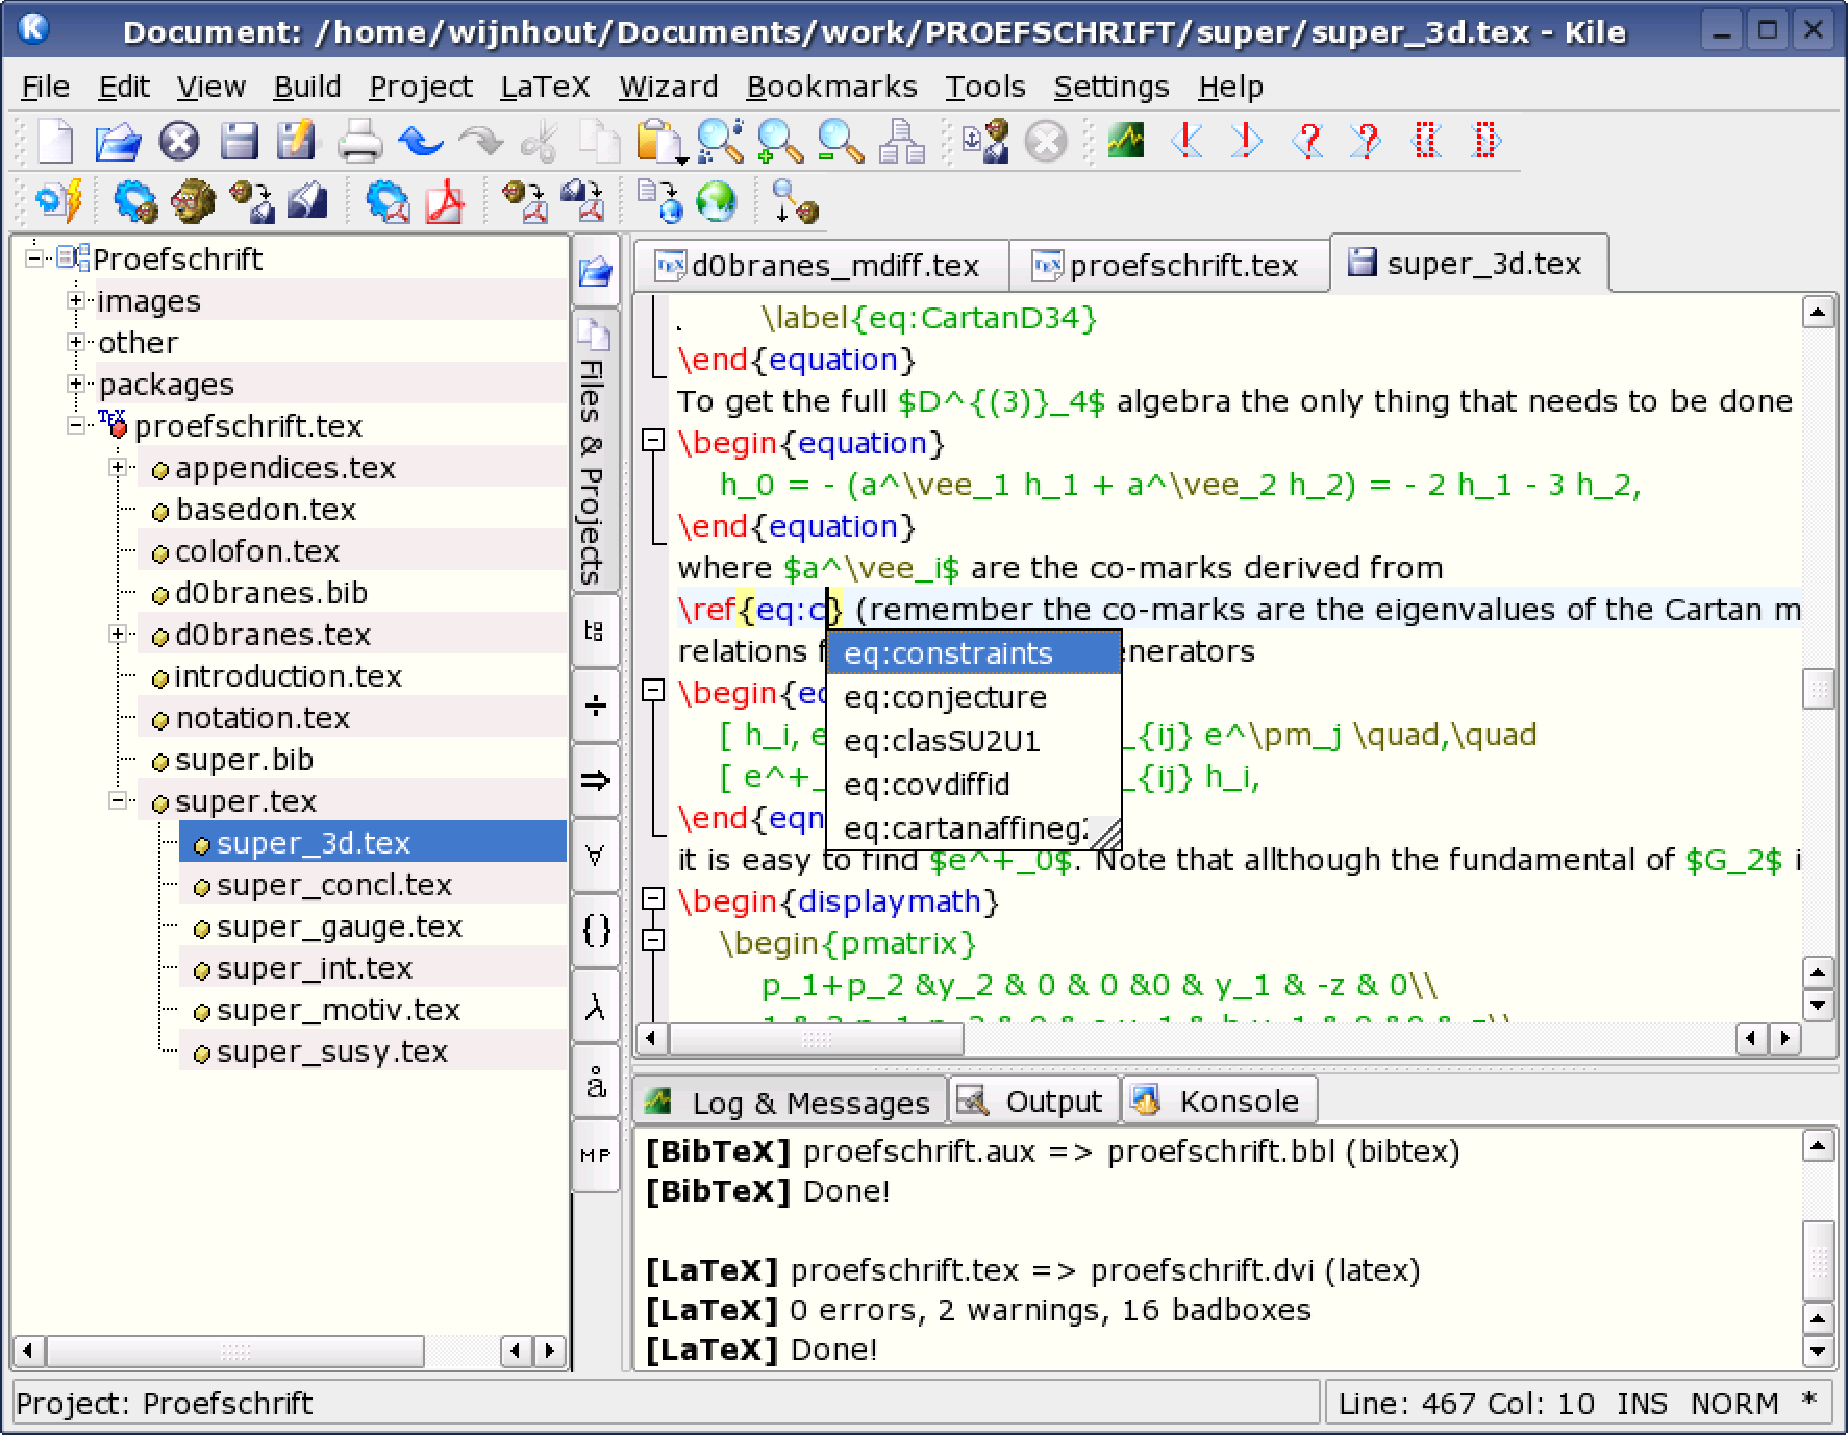
\includegraphics[width=13cm]{bilder/kile}
\caption{Bildschirmfoto {\ttfamily kile}}
\label{bild:kile}
\end{figure}

Kile organisiert mehrere Teildokumente zu einem Projekt und
bietet damit einen einfachen Zugriff auf alle Teildokumente
einer Ausarbeitung. Syntaxhighlighting ist ebenfalls vorhanden,
sowohl f�r \LaTeX als auch f�r die BibTex"=Literaturdatenbanken.
F�r den Start eines \LaTeX"=Durchlaufes sowie den verschiedenen
Konvertierungsm�glichkeiten gibt es einzelne Kn�pfe. Ein direktes
Hin- und Herspringen zwischen DVI- und TEX"=Ansicht, wobei
an die korrekte Stelle gesprungen wird, ist m�glich. Dies vereinfacht
Korrekturen speziell bei umfangreicheren Dokumenten.



\subsection{{\ttfamily TeXnicCenter} -- Windows}
Ein Bildschirmfoto von {\ttfamily TeXnicCenter} zeigt Abbildung
\ref{bild:texniccenter}.

\begin{figure}[!ht]
\centering
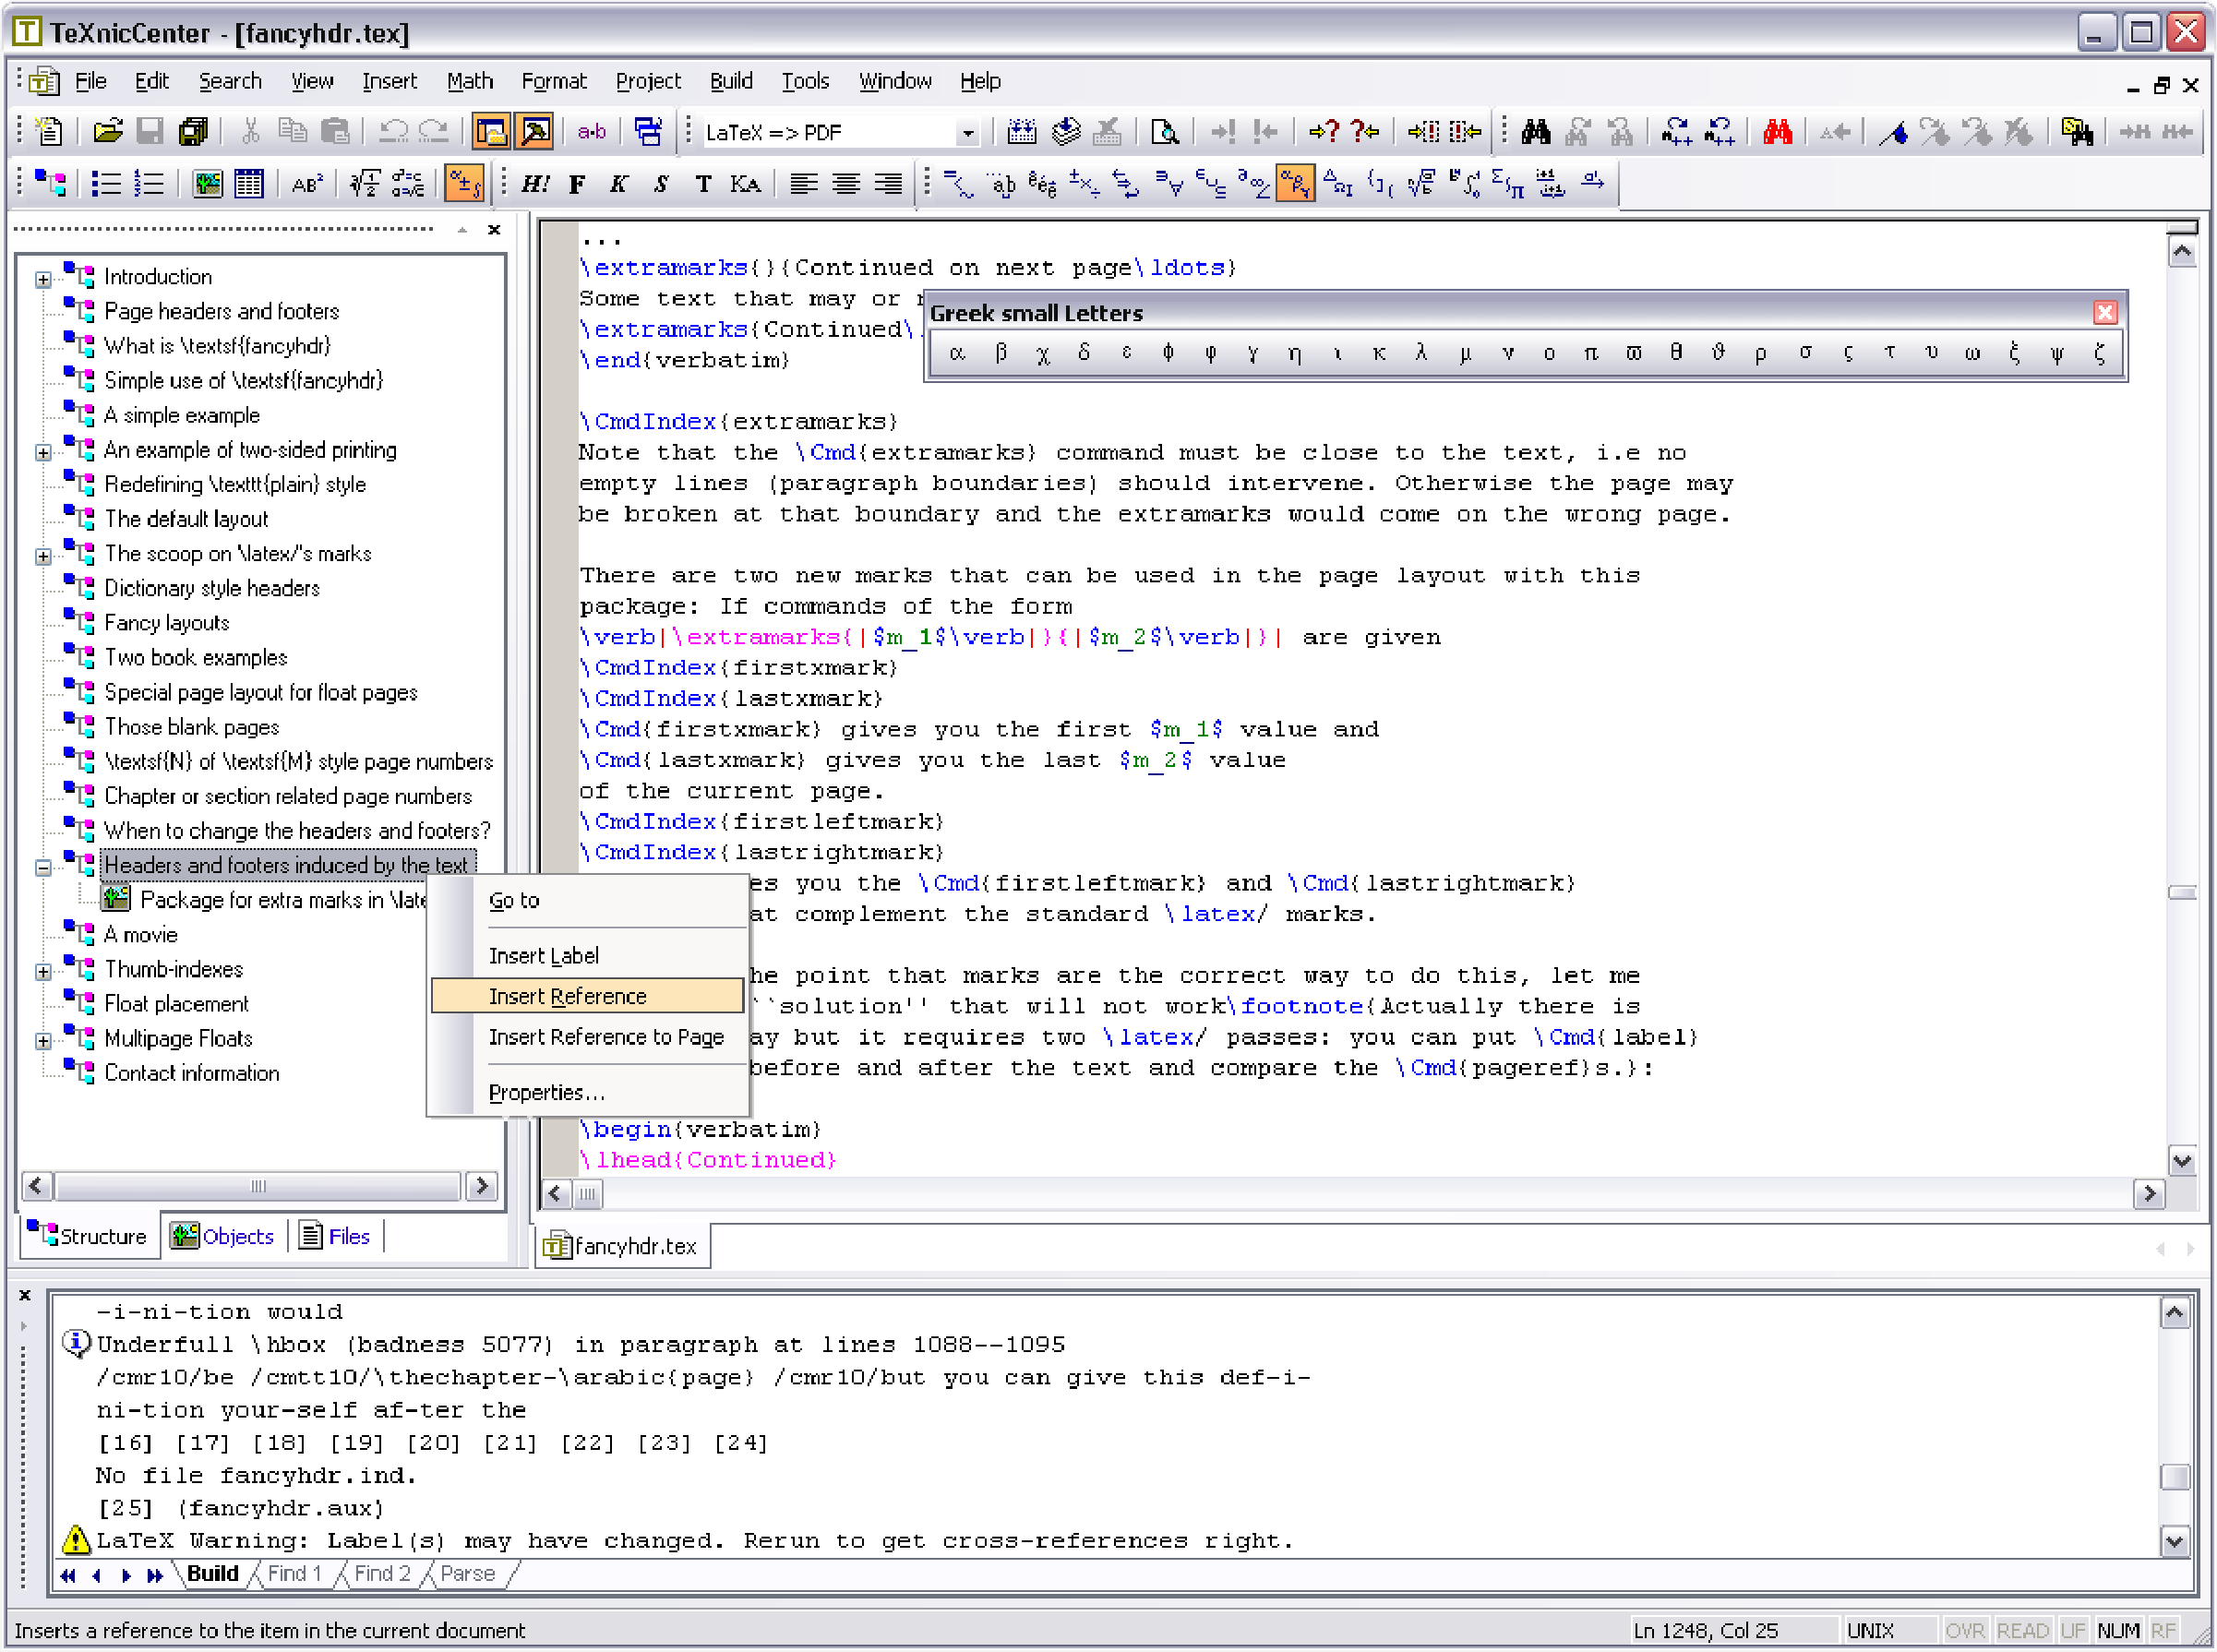
\includegraphics[width=13cm]{bilder/texniccenter}
\caption{Bildschirmfoto {\ttfamily texniccenter}}
\label{bild:texniccenter}
\end{figure}

Der Editor bietet Syntaxhighlighting f�r die verschiedenen
Latexbefehle. Kurz gesagt bietet diese Entwicklungsumgebung die
selben Features wie die im letzten Abschnitt vorgestellte
Software "`Kile."'



\section{Dateien dieser Formatvorlage}
Siehe Tabelle \ref{tabelle:dateien}.

\begin{table}[ht!]
\centering
\begin{tabular}{ll}
\hline
Dateiname &
Beschreibung
\\
\hline
{\ttfamily abschlusserklaerung.tex} &
\LaTeX\ Teildokument
\\
{\ttfamily anhang\_abbildungsverzeichnis.tex} &
\LaTeX\ Teildokument
\\
{\ttfamily anhang\_abkuerzungsverzeichnis.tex} &
\LaTeX\ Teildokument
\\
{\ttfamily anhang\_literaturverzeichnis.tex} &
\LaTeX\ Teildokument
\\
{\ttfamily anhang\_messwerte.tex} &
\LaTeX\ Teildokument
\\
{\ttfamily anhang\_programm\_a.tex} &
\LaTeX\ Teildokument
\\
{\ttfamily anhang\_programm\_b.tex} &
\LaTeX\ Teildokument
\\
{\ttfamily anhang\_protokoll.tex} &
\LaTeX\ Teildokument
\\
{\ttfamily anhang\_tabellenverzeichnis.tex} &
\LaTeX\ Teildokument
\\
{\ttfamily bilder/} &
Hier alle Bilder ablegen!
\\
{\ttfamily dokument.dvi} &
Ergebnis des \LaTeX\ Durchlaufes
\\
{\ttfamily dokument.pdf} &
Erzeugtes PDF"=Dokument
\\
{\ttfamily dokument.ps} &
Erzeugtes Postscript"=Dokument
\\
{\ttfamily dokument.tex} &
\LaTeX\ Hauptdokument
\\
{\ttfamily itmabbrv.bst} &
Formatvorlage
\\
{\ttfamily itmalpha.bst} &
Formatvorlage
\\
{\ttfamily kapitel1.tex} &
\LaTeX\ Teildokument
\\
{\ttfamily kapitel2.tex} &
\LaTeX\ Teildokument
\\
{\ttfamily kapitel3.tex} &
\LaTeX\ Teildokument
\\
{\ttfamily kurzfassung.tex} &
\LaTeX\ Teildokument
\\
{\ttfamily latexvorlage.kilepr} &
Projektdatei f�r {\ttfamily Kile}
\\
{\ttfamily latexvorlage.tcp} &
Projektdatei f�r {\ttfamily TeXnicCenter}
\\
{\ttfamily literatur.bib} &
Die Literaturdatenbank
\\
{\ttfamily thesen.tex} &
\LaTeX\ Teildokument
\\
{\ttfamily titelblatt.tex} &
\LaTeX\ Teildokument
\\
{\ttfamily vorwort.tex} &
\LaTeX\ Teildokument
\\
\hline
\end{tabular}
\caption{Relevante Dateien im Paket}
\label{tabelle:dateien}
\end{table}


\chapter{Planung}
\section{Entwürfe}
Da die Entscheidung für das finale Konzept sehr früh gefallen ist, wurde sich darauf geeinigt, dass zwei Gruppenmitglieder dieses Konzept bearbeiten, dafür aber viel tiefer ins Detail gehen. 
Die übrigen zwei Gruppenmitglieder haben jeweils eine eigene Idee behandelt, blieben dabei aber deutlich oberflächlicher. 

Insgesamt sind dabei die drei im Folgenden vorgestellte Konzepte entwickelt worden.

\subsection{Seggway}

\subsection{Weggchair}
Beim Weggchair ist die Namensgebung leider ein wenig misslungen. 
Der Rest vom Konzept wäre mit den vom Lehrstuhl bereitgestellten Materialien recht leicht zu realisieren gewesen.
Deswegen wäre es der Plan B gewesen, falls unser präferiertes Konzept nicht finalisiert werden kann. 

Das Konzept orientiert sich, wie der Name andeuten soll, recht nahe an einem Rollstuhl. 
Die gesamte Elektronik befindet sich in einer Zwischenebene unter der ``Sitzfläche''. 
Gelenkt wird der Weggchair indem sich beide Motoren verschieden schnell drehen. 

Wie in der Skizze (Abb.~\ref{bild:weggchair}) zu sehen, ist das ``Stützrad'' eher eine ``Stützkugel'', die in alle Richtungen über den Boden gleiten kann. 
Statt einer Kugel wäre auch eine oder zwei drehbar gelagerte Rollen denkbar gewesen, ähnlich wie bei einem Einkaufswagen oder natürlich dem Original. 

Da die verwendeten DC-Motoren unter Volllast über 7000 Umdrehungen schaffen, dafür aber weniger Drehmoment haben wäre, wie in der finalen Idee, ein Planetengetriebe innerhalb der großen Räder zum Einsatz gekommen. 

Das Ei wäre wäre beim Weggchair an der Stelle befestigt, wo normalerweise der Rollstuhlfahrer sitzt. Dafür wäre eine Federung und Halterung an dieser Stelle gewesen. Vermutlich wäre ein mit Watte oder einem ähnlichen elastischen, polsternden Material ausgestatteter Eierbecher zum Einsatz gekommen.

\begin{figure}[!ht]
	\centering
	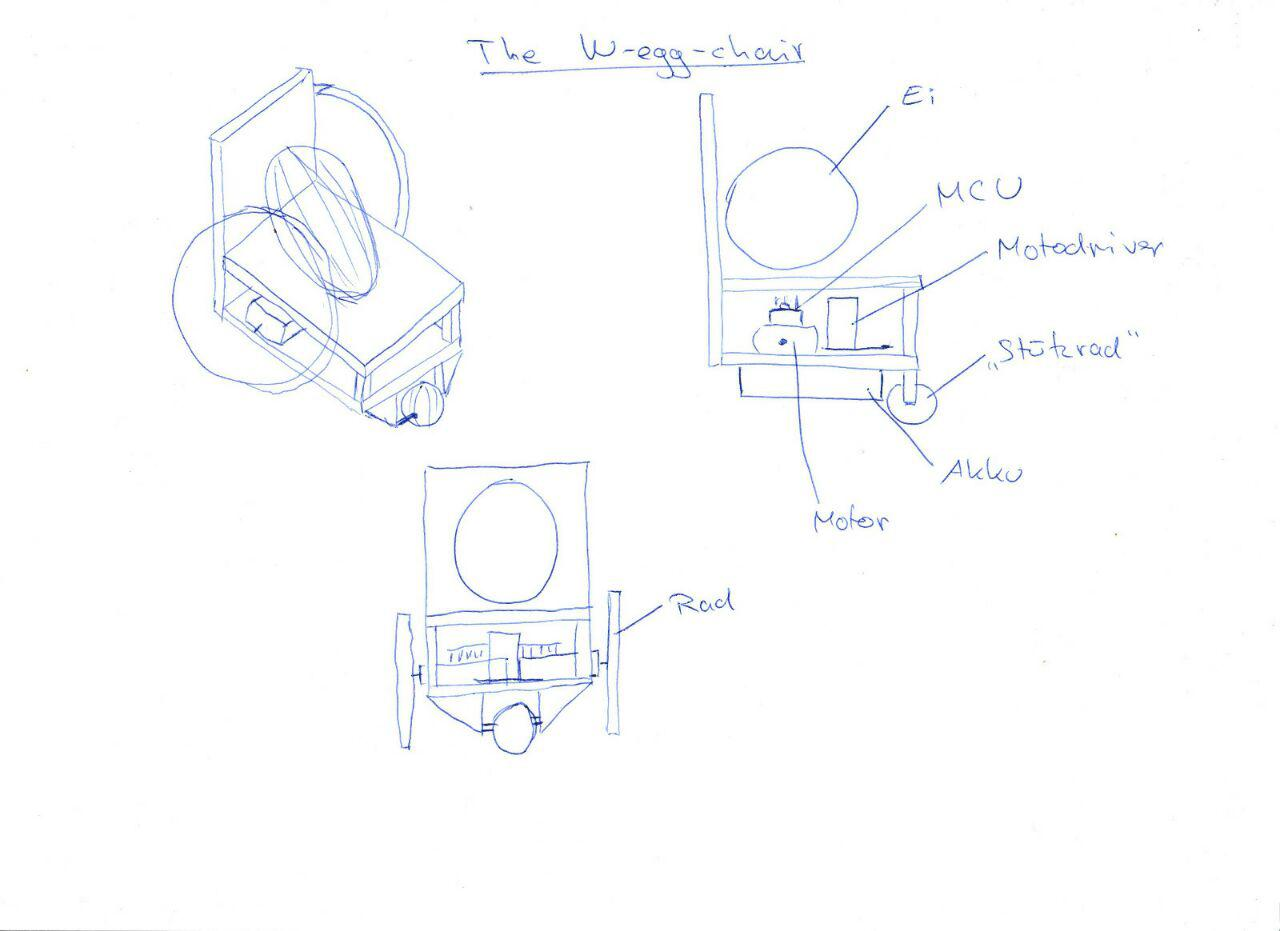
\includegraphics[width=\textwidth]{bilder/weggchair.jpg}
	\caption{Skizze Weggchair}
	\label{bild:weggchair}
\end{figure}


\subsection{TEGGLA}
Da sich die nächsten drei Kapitel nur mit dem finalen Konzept auseinandersetzen, wird an dieser Stelle nur ganz kurz auf das Konzept des TEGGLA (Abb.~\ref{bild:tegglaskizze}) eingegangen, damit die nachfolgenden Kapitel nachvollziehbar sind. 

Das besondere Feature beim TEGGLA sind die omnidirektionalen Räder, auch Mecanum bezeichnet, die neben dem normalen Vorwärtsfahren auch Seitwärtsbewegungen und Rotation zulassen. 
Diese drei Freiheitsgrade lassen sich auch beliebig kombinieren. 
Dadurch ist in der Ebene jede denkbare Richtung befahrbar. Dazu sind allerdings vier Motoren notwendig. 

Ergo wächst die Elektronikteileliste wie folgt: Für die zwei Extramotoren wird eine zusätzliche H-Brücke benötigt. 
Leider hat das bereitgestellte ESP-8266 nicht genug Pins für die zusätzliche Elektronik, weswegen zum ESP-32 upgegraded werden musste. 

Es folgen noch viel mehr Details, aber um die folgenden Kapitel zu verstehen muss noch gesagt werden, dass der TEGGLA in der Entwicklungsphase noch Omni-Move hieß. Beide Namen sind im Folgenden also synonym. 

\begin{figure}[!ht]
	\centering
	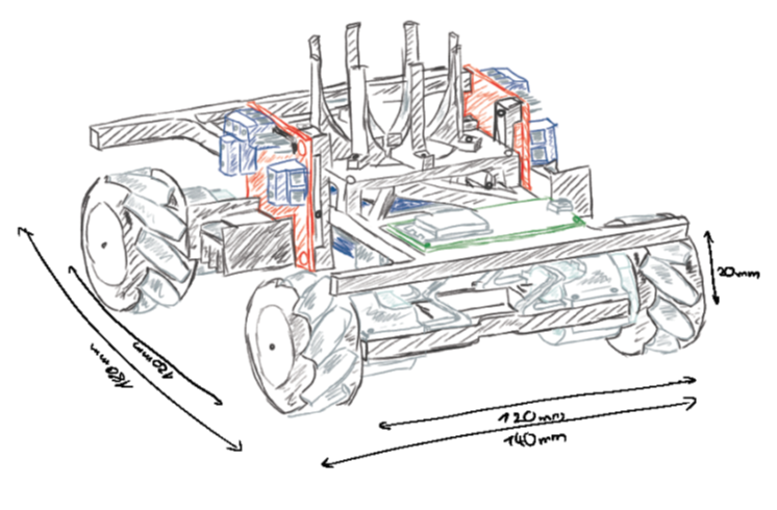
\includegraphics[width=\textwidth]{bilder/tegglaskizze.png}
	\caption{Skizze TEGGLA}
	\label{bild:tegglaskizze}
\end{figure}


\section{Morphologischer Kasten}
Mithilfe des Morphologischen Kasten (Abb.~\ref{bild:morphkasten}) lassen sich die benötigten Komponenten auf eine einfach ersichtliche Weise vergleichen.
\begin{figure}[H]
	\centering
	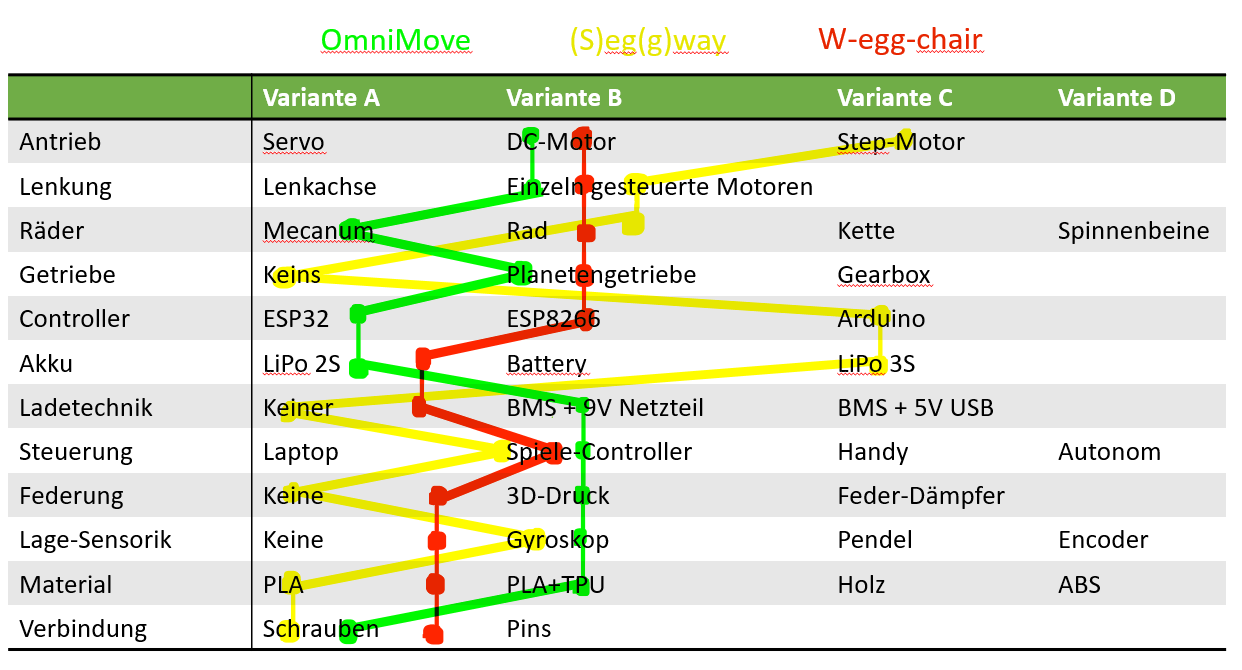
\includegraphics[width=\textwidth]{bilder/morphkasten.png}
	\caption{Morphologischer Kasten}
	\label{bild:morphkasten}
\end{figure}

\section{Online Bestellungen}
Um das Fahrzeug nach dem Praktikum behalten zu können, war eine Voraussetzung, dass nur Teile verbaut werden, die nicht Eigentum des Lehrstuhls sind.
Aus diesem wurden die nötigen Bauteile bei unterschiedlichen Onlineshops herausgesucht und bestellt.
Hierbei fiel die Entscheidung auf Pollin, einem deutschen Elektronik Händler und AliExpress, einem chinesischen Großhändler.
In der ursprünglichen Planung wurden die Kosten pro Fahrzeug auf circa \EUR{20} -- \EUR{25} überschlagen.
In der finalen Bestellung beliefen sich die Kosten auf insgesamt etwa \EUR{32}.

Siehe Tabelle~\ref{table:Kosten} für eine genaue Aufteilung der Kosten.
\begin{table}[!ht]
	\centering
\begin{tabular}{lcccc}
	Artikel & Stk & \euro/Stk & \euro{} & Laden\\
	\midrule[2pt]
	Netzteil 9V 1A & 1 & 0,95 & 0,95 & Pollin\\
	\midrule
	DC Motor & 4 & 0,95 & 3,80 & Pollin\\
	\midrule
	2S LiPo & 1 & 9,95 & 9,95 & Pollin\\
	\midrule
	XT60 5er Satz & 0,5 & 1,8 & 0,90 & AliExpress\\
	\midrule
	ESP32 & 1 & 3,77 & 3,77 & AliExpress\\
	\midrule
	2s BMS & 1 & 0,89 & 0,89 & AliExpress\\
	\midrule
	Kabelset 20cm & 0,5 & 3,30 & 1,65 & AliExpress\\
	\midrule
	Kabelset F -- F 10cm & 0,5 & 0,68 & 0,34 & AliExpress\\
	\midrule
	Gyroskop & 1 & 0,93 & 0,93 & AliExpress\\
	\midrule
	H-Brücken & 2 & 1,17 & 2,34 & Bestand\\
	\midrule
	Filament \textit{[kg]} & 0,05 & 20,00 & 1,00 & Bestand\\
	\midrule
	Schrauben + Muttern \textit{[Set]} & 1 & 1,00 & 1,00 & Bestand\\
	\midrule
	Motorkabel & 1 & 0,50 & 0,50 & Bestand\\
	\midrule
	Versandkosten AliExpress & 0,25 & 9,00 & 2,25 & \\
	\midrule
	Versandkosten Pollin & 0,25 & 5,00 & 1,25 & \\
	\midrule
	\midrule
	 &  & Total & \EUR{31,52} & \\
\end{tabular} 
\caption{Kostenübersicht} 
\label{table:Kosten}
\end{table} 

\section{Verwendete Technologien}

\subsection{Git}


\subsection{Creo}
Bei der CAD-Software standen mehrere unterschiedliche Programme unterschiedlicher Hersteller zur Auswahl.
Diese waren ``Catia'' von Dassault Systemes, ``Sketchup'' von Trimble Inc., ``Creo Parametrics'' von PTC Inc., ``Blender'' von Blender Foundation, ``OpenSCAD'' (Opensource Programm) und ``FreeCAD'' (ebenfalls Opensource).
Nach längerem Abwägen viel die Entscheidung auf das Programm Creo Parametrics, da dieses vergleichbar einfach zu bedienen ist, aber trotzdem einen sehr großen Funktionsumfang bietet.
Des weiteren bietet Creo eine gute 3D-Maus Unterstützung, was das Modellieren deutlich vereinfachte.
Trotz des großen Funktionsumfangs reichten die Möglichkeiten, die Creo bietet, nicht immer aus, weshalb in Einzelfällen auf andere CAD-Programme zurückgegriffen wurde. Diese werden allerdings an den betroffenen Stellen extra erwähnt. 

\subsection{PlatformIO}
Die Wahl der Entwicklungsumgebung fiel auf Visual Studio Code mit PlatformIO, anstelle von der in der Vorlesung vorgestelleten Arduino IDE.

Mit der extremen Erweiterbarkeit von VSCode ist hier die Programmierung einfacher und fehlerfreier durchzuführen, da in Arduino IDE nur bedingtes Syntax-checking vorhanden ist.

Durch PlatformIO stellt sich Einbingen von externen Bibliotheken ebenfalls als Leichtigkeit heraus.
Desweiteren ist hier die Unterstützung von einer Vielzahl von MicroControllern bereits integriert.
\chapter{Entwicklung der Schlüsselelemente}
\section{Übersicht des gesamten Modells}

\section{Schaltplan}

\section{BMS und Laden}

\section{Mecanum}

\section{Planetengetriebe}

\section{ESP-32 vs. ESP-8266}
Bei dem vom Lehrstuhl gestellten ESP-8266 handelt es sich um ein WiFi-fähigen Microcontroller der chinesischen Firma ``espressif''.
Dieser besitzt 17 GPIO Pins, wovon jedoch lediglich 11 Pins nutzbar sind, da 6 an den externen SPI Flash angeschlossen sind.
Da dies wie in Tabelle~\ref{table:pins} aufgezeigt nicht für unsere Zwecke reicht, musste auf den leistungsstärkeren ESP-32 ausgewichen werden.

\begin{table}[!ht]
\centering
\begin{tabular}{lr}
	\multicolumn{2}{c}{Benötigte Pins} \\ 
	\midrule[3pt] 
	4x PWM & Motor Enable \\ 
	\midrule 
	8x Output & Motor Richtung \\ 
	\midrule 
	2x I$^2$C & Gyroskop \\ 
	\midrule 
	1x ADC & Batteriespannung \\ 
	\midrule
	\midrule 
	\multicolumn{2}{c}{15 Pins} \\ 
	 
\end{tabular} 
\caption{Aufzählung benötigter Pins} 
\label{table:pins}
\end{table} 

Obwohl die Anzahl der Pins das ausschlaggebenede Argument für einen Austausch des MicroControllers war, bringt dieser natürlich weitere Vorteile mit sich.

Beispielsweise profitiert die später genauer erklärte Website stark davon, auf einen zweiten Core ausgelargert werden zu können.

Siehe Tabelle~\ref{table:esp32} für einen Vergleich der beiden MicroController anhand der für dieses Projekt relevanten Faktoren.


\begin{table}[!ht]
\centering	
\begin{tabular}{lcc}
	& ESP-8266 & ESP-32 \\ 
	\midrule[3pt]
	Cores & single core & dual core \\ 
	\midrule
	Max Frequenz & 160 MHz & 240 MHz \\ 
	\midrule 
	\textbf{GPI} & \textbf{17 (11 nutzbar)} & \textbf{36 (30 nutzbar)} \\ 
	\midrule
	SRAM & 160 KB & 520 KB \\ 
	\midrule
	ADC Auflösung & 10 bit & 12 bit \\ 
	\midrule
	Stromverbrauch & 80 mA & 260 mA \\ 
	\midrule
	Preis (aus China) & \EUR{2} & \EUR{4} \\ 
\end{tabular} 
\caption{Vorteile des ESP-32} 
\label{table:esp32}
\end{table} 


\section{User-Interface}
\subsection{Java (obsolet)}

\subsection{HTML5 und Controller-Anbindung}

Das Java Programm wurde aus mehreren Gründen zugunsten einer auf HTML5, sowie JavaScript basierten Weboberfläche ersetzt:\par

\begin{itemize}
	\item Native und einheitliche Unterstützung für Controller unterschiedlichster Marken in HTML5\par
	
	\item Unabhängig von Java Laufzeitumgebung, sowie Verfügbarkeit des Programms.\\
	(Hierbei muss nur ein Browser auf dem PC installiert sein.)\par
	
	\item Einfache Übertragung der Daten per WebSockets anstatt von ``ra''  Sockets, ohne ein eigenes ``Frame'' um die Daten bauen zu müssen
\end{itemize}\par


\vspace{\baselineskip}
Dies lässt sich sehr leicht durch die ESPAsyncWebServer Library für den ESP32 lösen. \par

Diese hostet direkt auf dem ESP32 einen WebServer der sowohl HTML5, JS, als auch CSS bereitstellen kann. Als Speicherort für diese Dateien wird das sogenannte Dateisystem SPIFFS verwendet, welches den Flashspeicher des ESP32 als Dateisystem benutzt, wie es beispielsweise aus Windows bekannt ist.\par

Eine Einschränkung ist die Limitierung auf eine gleichzeitige Verbindung zu dem Server. Dies wurde empirisch herausgefunden und somit konnte nicht sicher gesagt werden, ob es sich hier um eine Einschränkung aufgrund von mangelnder Rechenleistung handelt oder ob die Library nicht mehr unterstützt. Als Lösung dieses Problems, ist nun die Anzahl der Verbindungen die der WiFi Accesspoint akzeptiert, auf eins gesetzt.\par


\vspace{\baselineskip}

\begin{figure}[!ht]
	\centering
	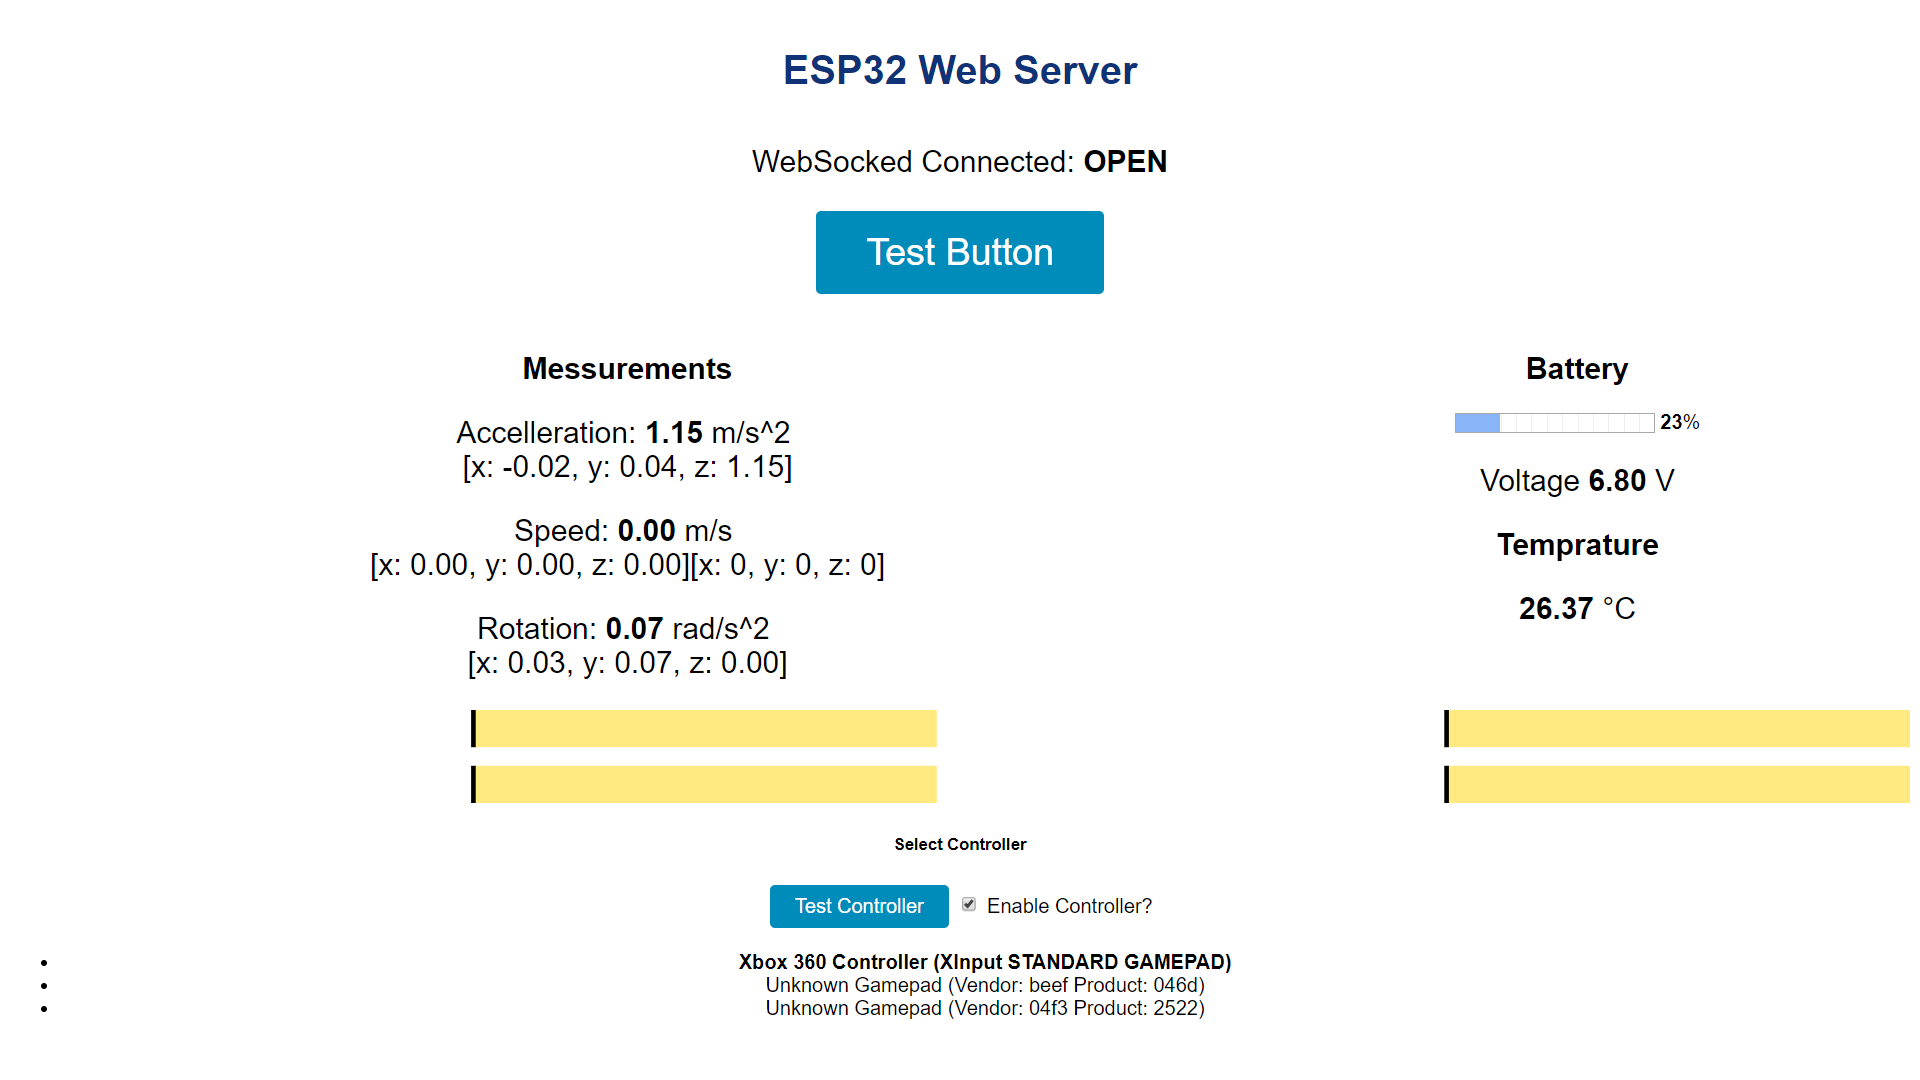
\includegraphics[width=\textwidth]{bilder/WebValues.png}
	\caption{Bildschirmfoto Weboberfläche}
	\label{bild:webvalues}
\end{figure}

In der Weboberfläche (Abb.~\ref{bild:webvalues}) sind ebenfalls noch jegliche Messwerte hinterlegt, die das Fahrzeug sammelt.\par

Diese sind:\par

\begin{itemize}
	\item Beschleunigung 
	\item Geschwindigkeit
	\item Rotationsgeschwindigkeit
	\item Batteriespannung
	\item Temperatur
	\item Drehgeschwindigkeit der jeweiligen Motoren
\end{itemize}\par


\vspace{\baselineskip}
Für die Wahl des Controllers ist eine auswählbare Liste aller angeschlossenen Controller am Ende der Seite vorhanden. Falls der Nutzer keinen Controller besitzt oder angeschlossen hat, kann durch das Abwählen der Checkbox auf die Steuerung per WASD, sowie die Pfeiltasten gewechselt werden.\par

\subsection{Protokoll}
Zum Übertragen wurde ein binäres Protokoll (Tabelle~\ref{table:protokoll}) entwickelt, um die Datenrate gering zu halten, sowie die Verarbeitung auf dem Microcontroller zu vereinfachen.\par

Da durch Websockets bereits ein Integrierter Frame geschickt wird, muss nicht bei jeder Nachricht die Länge und Anfangs- und Endbyte mitgeschickt werden, wie es sonst bei raw Sockets nötig gewesen wäre.\par

Hierbei wird jeder Wert als Int16 geschickt, um ein ausreichend großes Spektrum bei geringer Datenrate zu gewährleisten. \par

Am Anfang jeder Nachricht wird die ID ebenfalls als int16 geschickt, somit wären 65536 unterschiedliche Nachrichten erlaubt.\par

Um die Anzahl an Nachrichten zu verringern, wurden die Batteriespannung und Werte des Gyroskop zu einer kombinierte Nachricht zusammengefasst, um den Overhead gering zu halten.\par

\begin{table}[ht]
	\centering
	\resizebox{\textwidth}{!}{
\begin{tabular}{|c|c|c|c|c|c|c|c|c|c|c|c|c|}
	\hline 
	\textbf{Name} & \textbf{ID} & \multicolumn{11}{c|}{\textbf{Werte}} \\ 
	\hline 
	\hline 
	DRIVE & 0 & X-Achse L & Y-Achse L & X-Achse R & Y-Achse R &  &  &  &  &  &  &  \\ 
	\hline 
	GYRO & 1 & Speed-X & Speed-Y & Speed-Z & Accel-X & Accel-Y & Accel-Z & Rot-X & Rot-Y & Rot-Z  &  & \\ 
	\hline 
	BATTERY & 2 & Voltage &  &  &  &  &  &  &  &  &  &  \\ 
	\hline 
	MOTOR & 3 & Speed-M1 & Speed-M2 & Speed-M3 & Speed-M4 &  &  &  &  &  &  &  \\ 
	\hline 
	COMB & 4 & Speed-X & Speed-Y & Speed-Z & Accel-X & Accel-Y & Accel-Z & Rot-X & Rot-Y & Rot-Z  & Battery & Temp \\ 
	\hline 
\end{tabular}} 
\caption{Binäres Protokoll} 
\label{table:protokoll}
\end{table} 



\section{Steuerung per (XBox) Controller}
Wie bereits in der Dokumentation der Weboberfläche erwähnt, wird die Steuerung primär per Spiele Controller gelöst, beispielsweise einen XBox-Controller von Microsoft.
Diese Entscheidung ist in der erhöhten Mobilität motiviert. 

Mit einer Stuerung per WASD bzw. per Pfeiltasten sind nur binäre Zustände messbar, gedrückt oder nicht gedrückt, volle Geschwindigkeit oder Stillstand.
Im Vergleich dazu erlauben uns die JoySticks des Controllers durch unterschiedlich stare Auslenkung die Geschwindigkeit sehr variabel zu bestimmen.

Da hierbei ebenfalls der JoyStick in jegliche Richtungen bewegt werden kann, können ebenfalls die Mecanum Räder so angesteuert werden, dass sie in genau diese Richtung fahren.

Jedoch sind hiermit nur zwei der drei Freiheitsgrade unserer Fahrzeugs abgedeckt. Um Rotationen um die eigene Achse mit variabler Geschwindigkeit zu steuern, wird die Eingabe des linken und des rechten JoySticks mit folgenden Formelen überlagert.

\bigskip
Sei hier $controlSide$ Auslenkung des linken Sticks in X Richtung (nach rechts), 
$controlFront$ Auslenkung des linken Sticks in Y Richtung (nach vorne) und 
$controlTurn$ Auslenkung des rechten Sticks in X Richtung (nach rechts), 

\begin{align}
	\phi = atan2(controlSide, controlFront)\\
	vd = min(\sqrt{controlFront^2 + controlSide^2}, 1023) - \frac{controlTurn}{2}\\
	vphi = \frac{controlTurn}{2}
\end{align}


\section{PLA vs. TPU}

\section{Eierhalter}					

\section{Leichtbau}	
\chapter{Zukünftige Entwicklungsmöglichkeiten}
\section{Regler}

\section{Verbesserungen}
\subsection{Hardware}

\subsection{Software}

\chapter{Zusammenfassung}
In diesem abschließenden Kapitel werden die gesammelten Erfahrungen reflektiert, sowie die wichtigsten erlernten, beziehungsweise verbesserten Fähigkeiten beim Entwickeln des TEGGLA zusammengefasst.


\section{Fazit}
Das Entwickeln des TEGGLA hat dem gesamten Team sehr viel Spaß gemacht.
Um das erwünschte Ergebnis zu erreichen, wurde der Umgang mit vielen neuen Technologien erlernt beziehungsweise das bereits vorhandene Wissen vertieft. 
Vor allem das Konstruieren in CAD, die Anfertigung von technischen Zeichnungen und das tatsächliche Drucken und Zusammenbauen der Baugruppen hatten einen großen Mehrwert für unsere zukünftigen Projekte. 
Die wichtigsten verwendeten Technologien waren:

\subsection*{Creo}
Konstruieren aller Bauteile des TEGGLA.

\subsubsection*{C++}
Programmierung des MicroController auf einer Hardwarenahen Ebene.

\subsubsection*{JavaScript / HTML5}
Weboberfläche mit Sockets für die Kommunikation und Steuerung des TEGGLA.

\subsubsection*{Github}
Repository für die Sicherung, Versionierung, Verteilung und Aktualsierung aller Daten, technischen Zeichnungen, Skizzen, Berichte, Präsentationen und Quellcode.


\section{Errungene Erfahrung}
Der wohl zeitaufwändigste und schwierigste Aspekt des Projekts war der 3D-Druck eines Planetengetriebes, welches die erforderliche Übersetzung für das omnidirektionale Fahren bereitstellen kann. Bereits geringe Druckerungenauigkeiten führten zu nicht nutzbaren Getriebeversionen und daher wurden viele Anläufe benötigt, um ein passendes Planetengetriebe zu entwickeln. Für zukünftige Projekte mit 3D-Druckern wird das berücksichtigt und der Fokus bei der Entwicklung darauf gelegt.  

Als sehr positiv war die zeitliche Planung und Zusammenarbeit des Teams zu bewerten. Trotz unerwarteten Mehraufwänden für Teilaufgaben, kam es zu keinerlei zeitlichen Engpässen und dadurch zu einem qualitativ hochwertigen Endprodukt. Eine möglichst präzise Aufgabendefinition und -verteilung am Projektanfang ist enorm wichtig, um dies sicherstellen zu können. Zusätzlich waren die Meilensteintermine des Lehrstuhls ebenfalls hilfreich, um sich an den Terminplan zu halten.

Die Nutzung eines GIT Repositories war ebenfalls äußerst gewinnbringend, da die Versionierung, Verteilung, Aktualisierung und Sicherung jederzeit und für alle Teammitglieder gewährleistet werden konnte. 

Insgesamt wurden enorm viele Erfahrungen über den Entwicklungsprozess eines lenkbaren Fahrzeugs gesammelt, welche sich natürlich auch auf andere Produkte und Projekte abstrahieren lassen. Die einzelnen Entwicklungsschritte, nämlich die Auswahl einer Idee, das Anfertigen eines Lastenhefts, die Rollen- und Aufgabenverteilung innerhalb des Teams sowie die zeitliche Einhaltung von Terminen sind alles wichtige Kenntnisse für unsere zukünftigen Projekte.




\appendix
\part*{Anhang}
\chapter{Quellcode}

\section{ESP32}
\includeC{../../Arduino/OmniMoveESP/src/communication.cpp}{communication.cpp}
\includeC{../../Arduino/OmniMoveESP/src/communication.h}{communication.h}

\includeC{../../Arduino/OmniMoveESP/src/movement.cpp}{movement.cpp}
\includeC{../../Arduino/OmniMoveESP/src/movement.h}{movement.h}

\includeC{../../Arduino/OmniMoveESP/src/util.cpp}{util.cpp}
\includeC{../../Arduino/OmniMoveESP/src/util.h}{util.h}

\includeC{../../Arduino/OmniMoveESP/src/main.cpp}{main.cpp}

\section{Webpage}
\includeLang{../../Arduino/OmniMoveESP/data/index.html}{index.html}{html}
\includeLang{../../Arduino/OmniMoveESP/data/code.js}{code.js}{java}
\includeLang{../../Arduino/OmniMoveESP/data/style.css}{style.css}{java}

\section{Java}
\includeLang{../../Code_GUI/ProduktionstechnikPraktikum/src/main/ConnectUI.java}{main/ConnectUI.java}{java}

\includeLang{../../Code_GUI/ProduktionstechnikPraktikum/src/components/SpeedMeter.java}{components/SpeedMeter.java}{java}
\includeLang{../../Code_GUI/ProduktionstechnikPraktikum/src/Toaster/Toaster.java}{Toaster/Toaster.java}{java}
\includeLang{../../Code_GUI/ProduktionstechnikPraktikum/src/Toaster/ToasterBody.java}{Toaster/ToasterBody.java}{java}
\includeLang{../../Code_GUI/ProduktionstechnikPraktikum/src/Utils/UIUtils.java}{Utils/UIUtils.java}{java}
\includeLang{../../Code_GUI/ProduktionstechnikPraktikum/src/Utils/TextFieldIP.java}{Utils/TextFieldIP.java}{java}
\includeLang{../../Code_GUI/ProduktionstechnikPraktikum/src/Utils/TextFieldPort.java}{Utils/TextFieldPort.java}{java}
\includeLang{../../Code_GUI/ProduktionstechnikPraktikum/src/zweitesFenster/Main.java}{main/Main.java}{java}
\includeLang{../../Code_GUI/ProduktionstechnikPraktikum/src/zweitesFenster/ZweitesFenster.java}{main/ZweitesFenster.java}{java}

\chapter{Technische Zeichnungen}

\begin{figure}[ht!]
	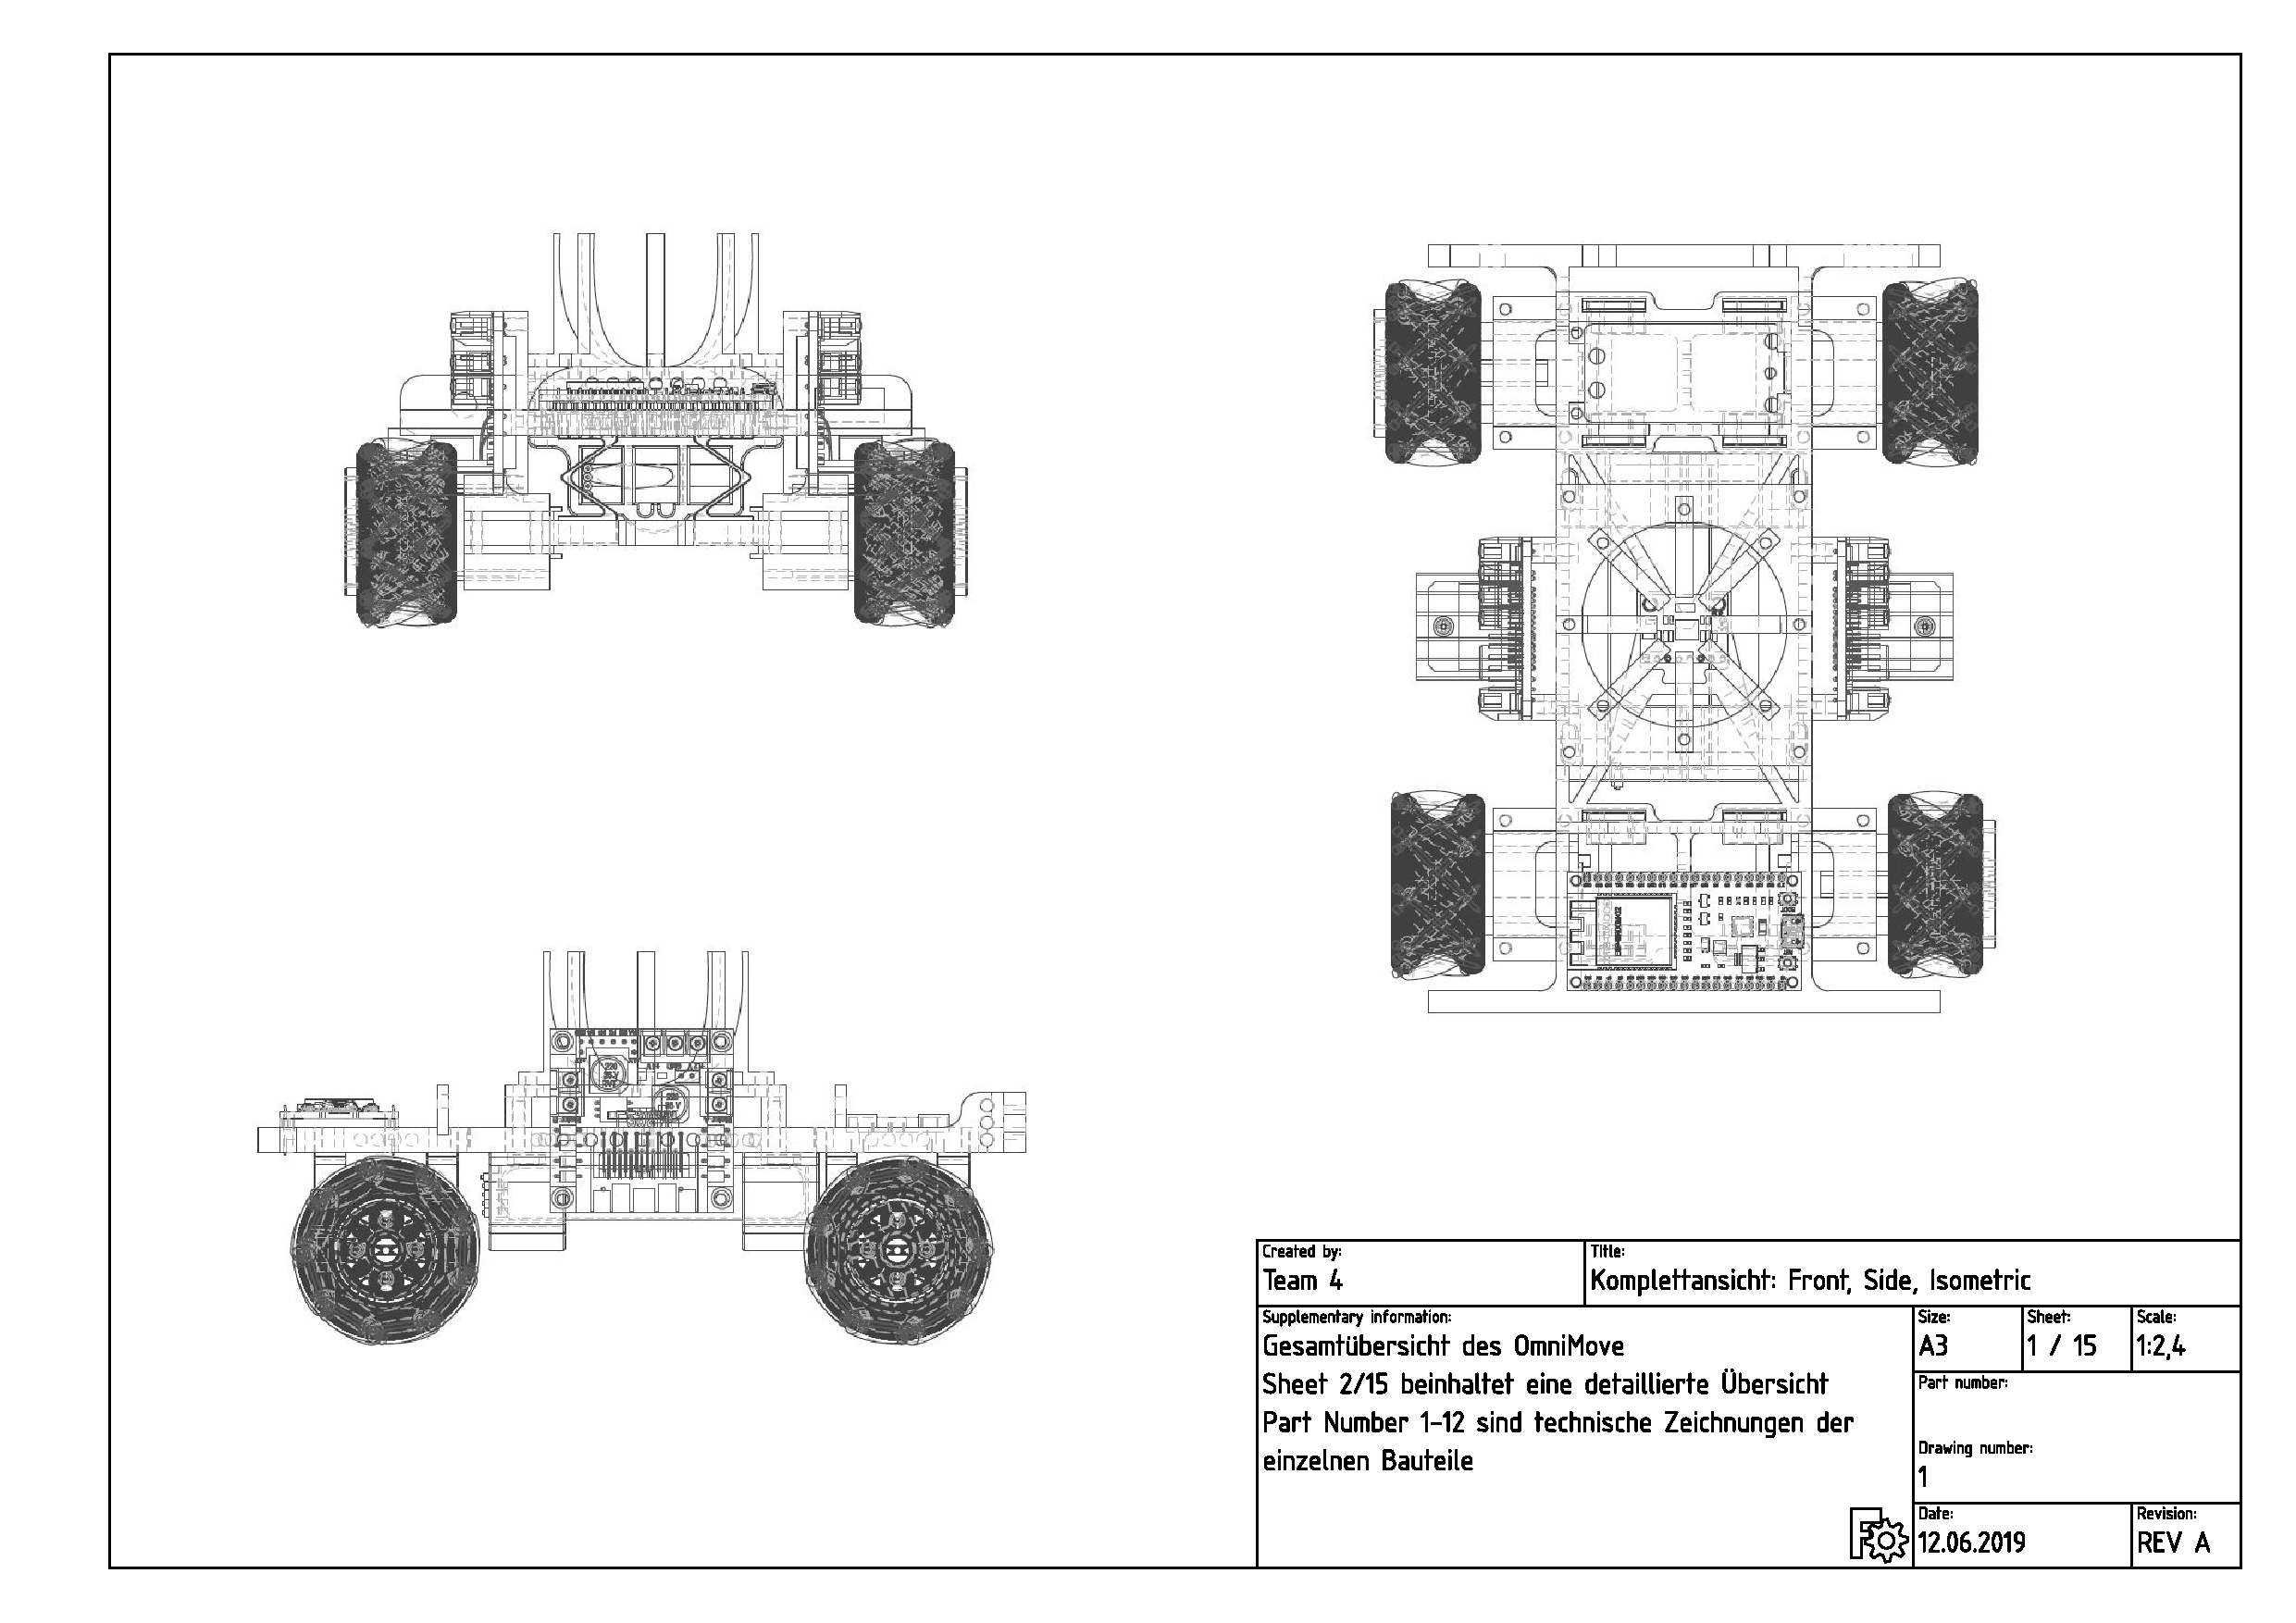
\includegraphics[width=\textwidth]{../techzeich/00.PDF} 	
	\caption{Komplettansicht}
\end{figure}

\begin{figure}[ht!]
	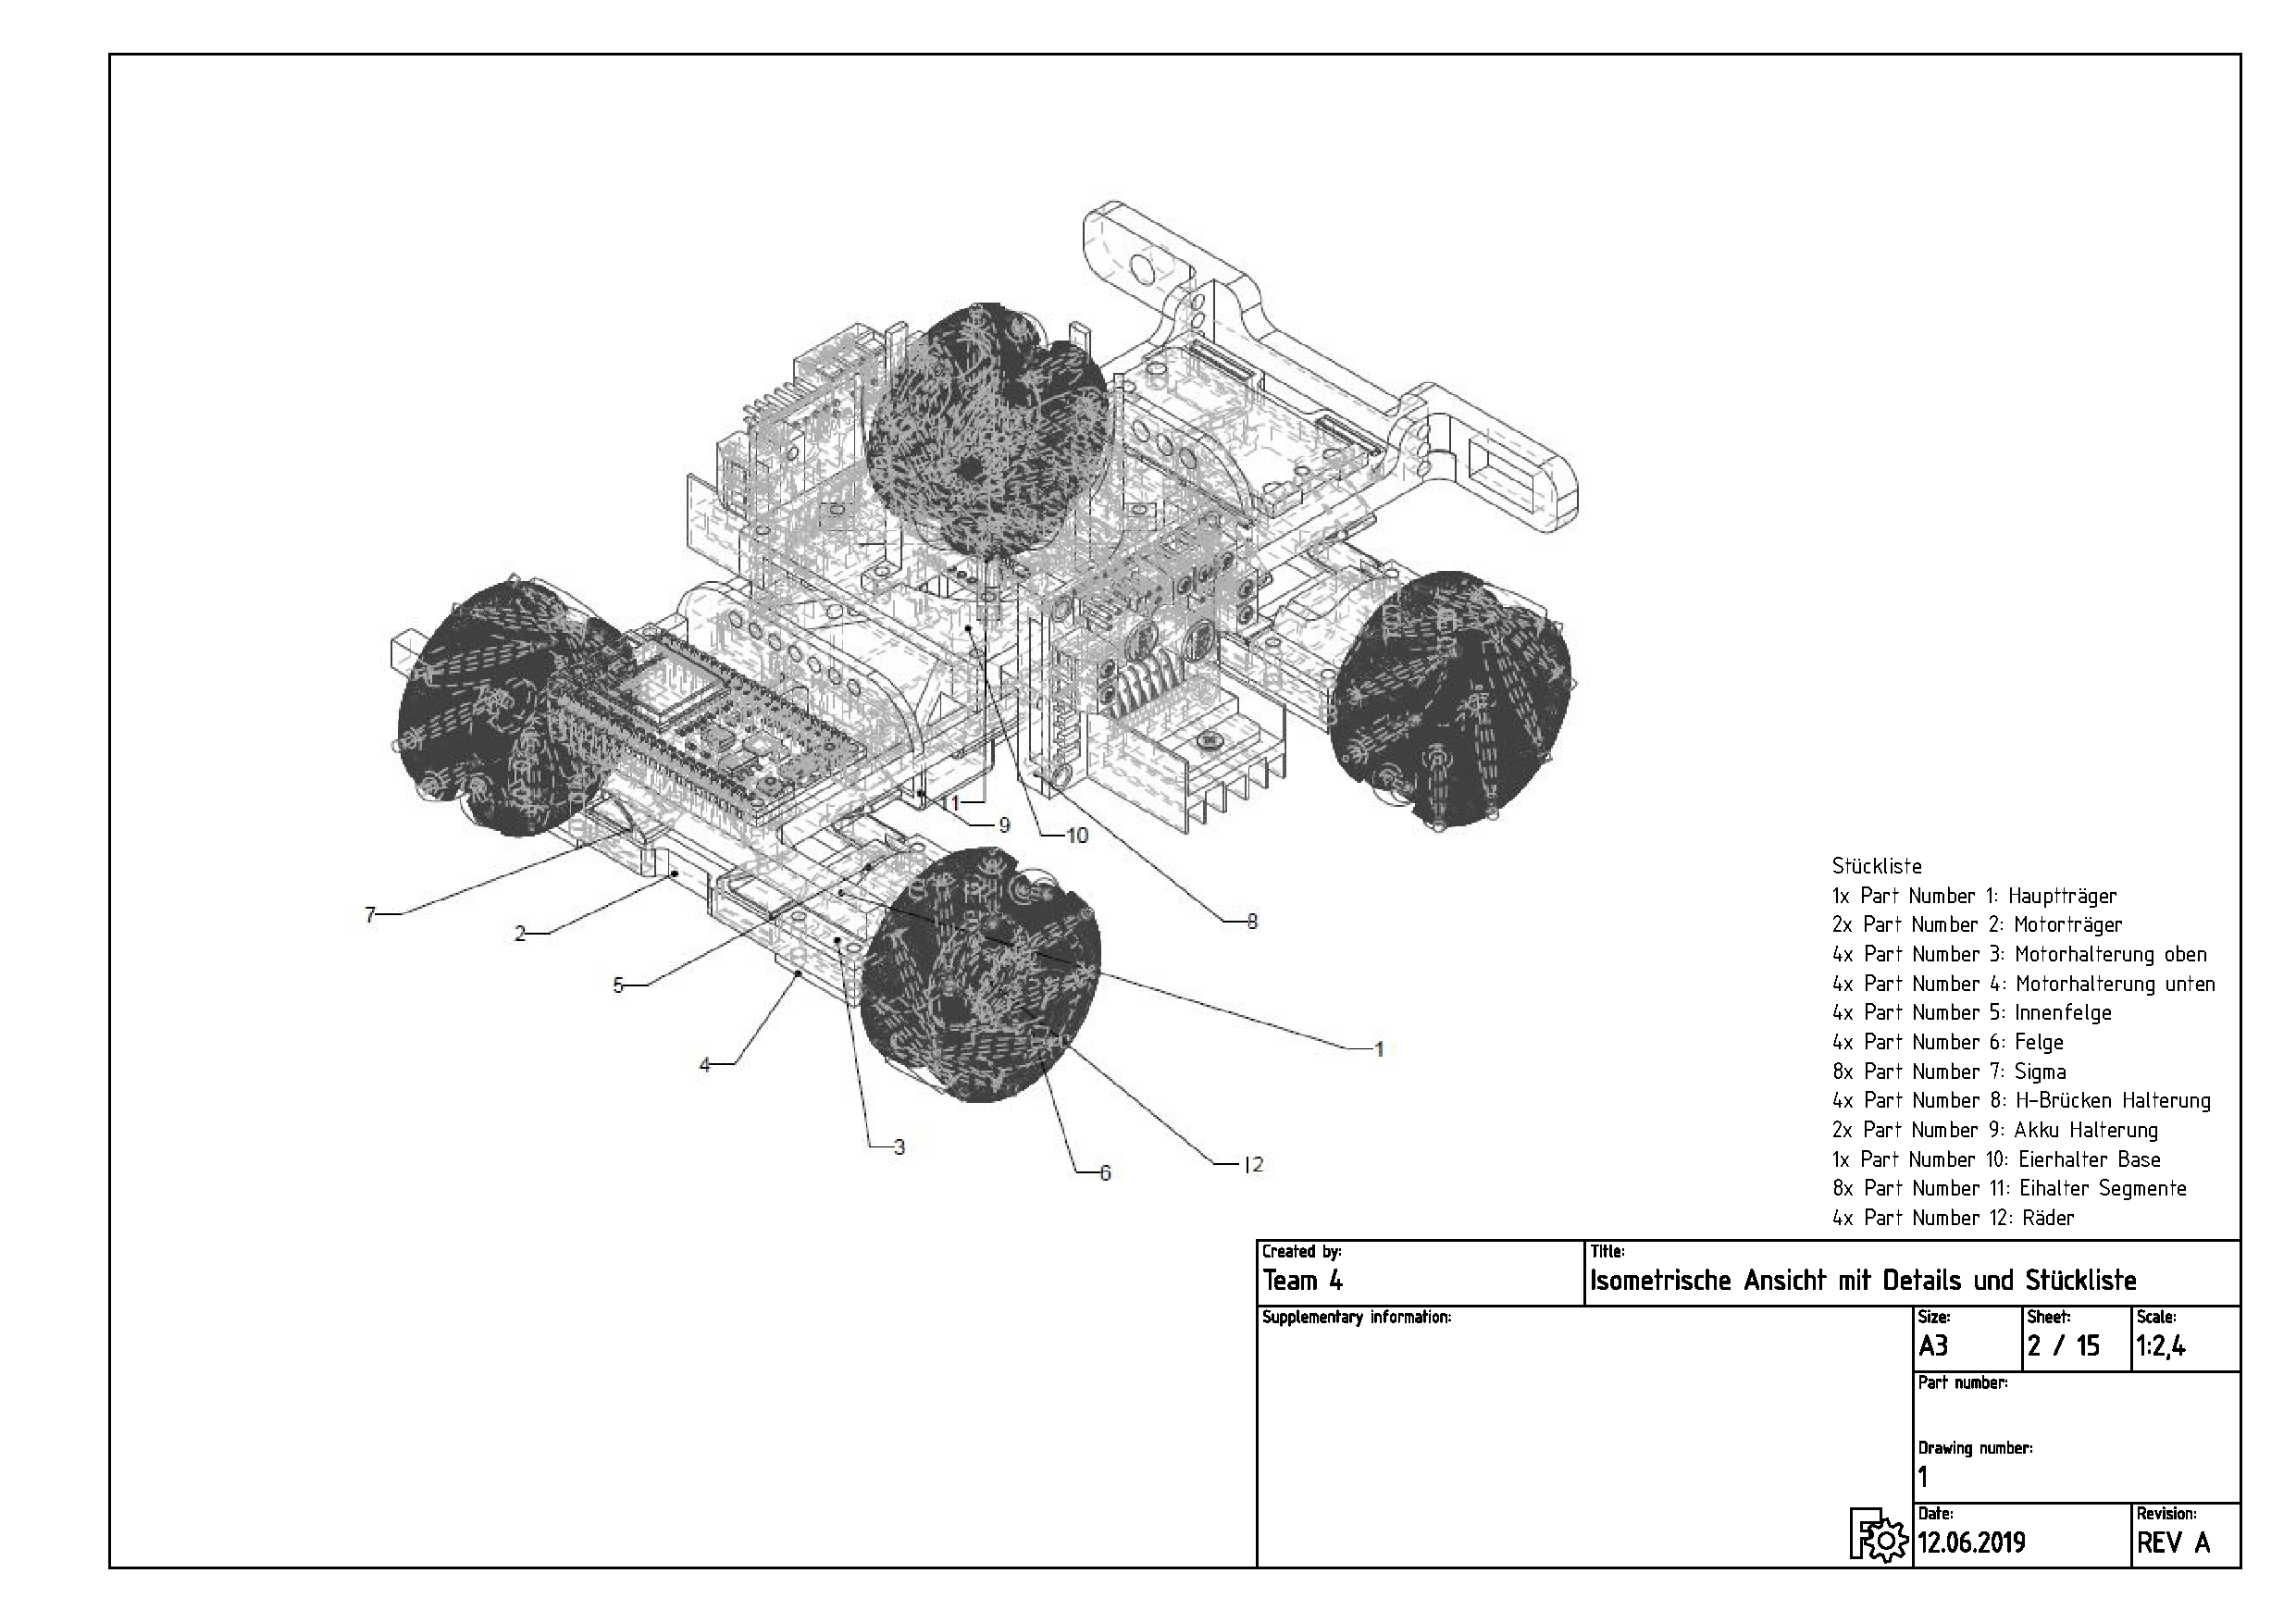
\includegraphics[width=\textwidth]{../techzeich/01.PDF} 
	\caption{Isometrisch und St�ckliste}
\end{figure}

\begin{figure}[ht!]
	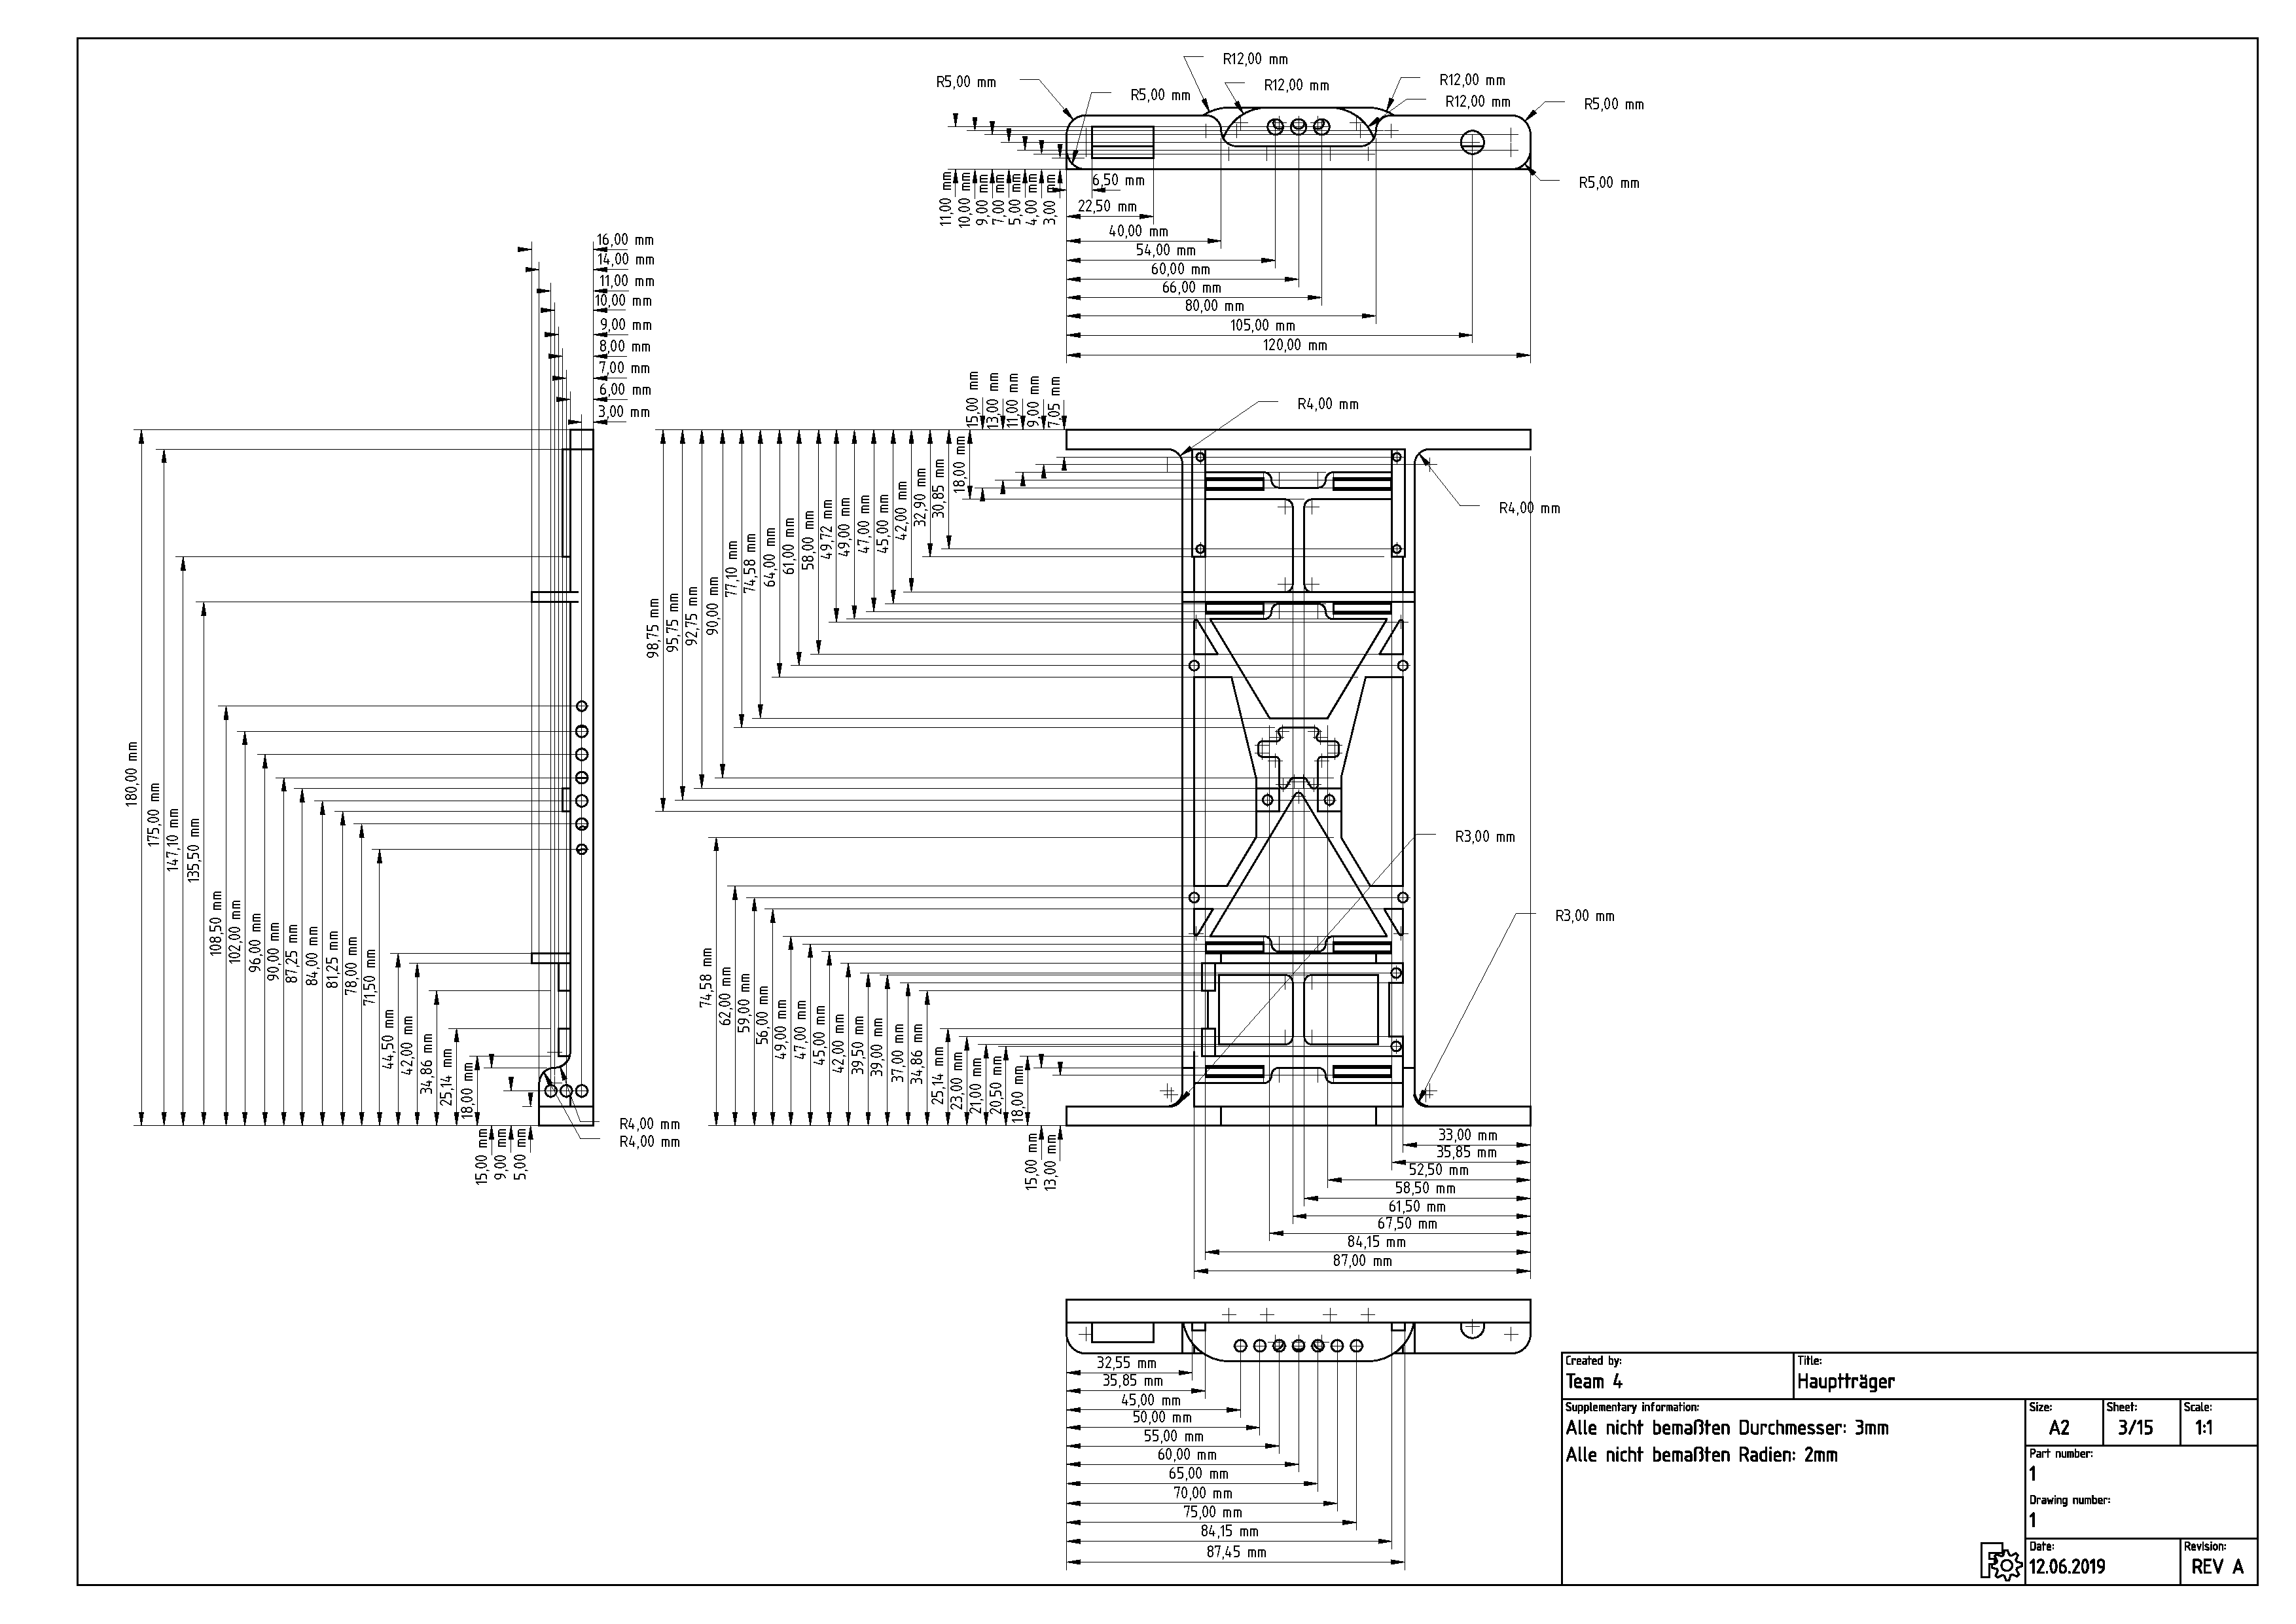
\includegraphics[width=\textwidth]{../techzeich/1.PDF} 	
	\caption{Haupttr�ger}
\end{figure}

\begin{figure}[ht!]
	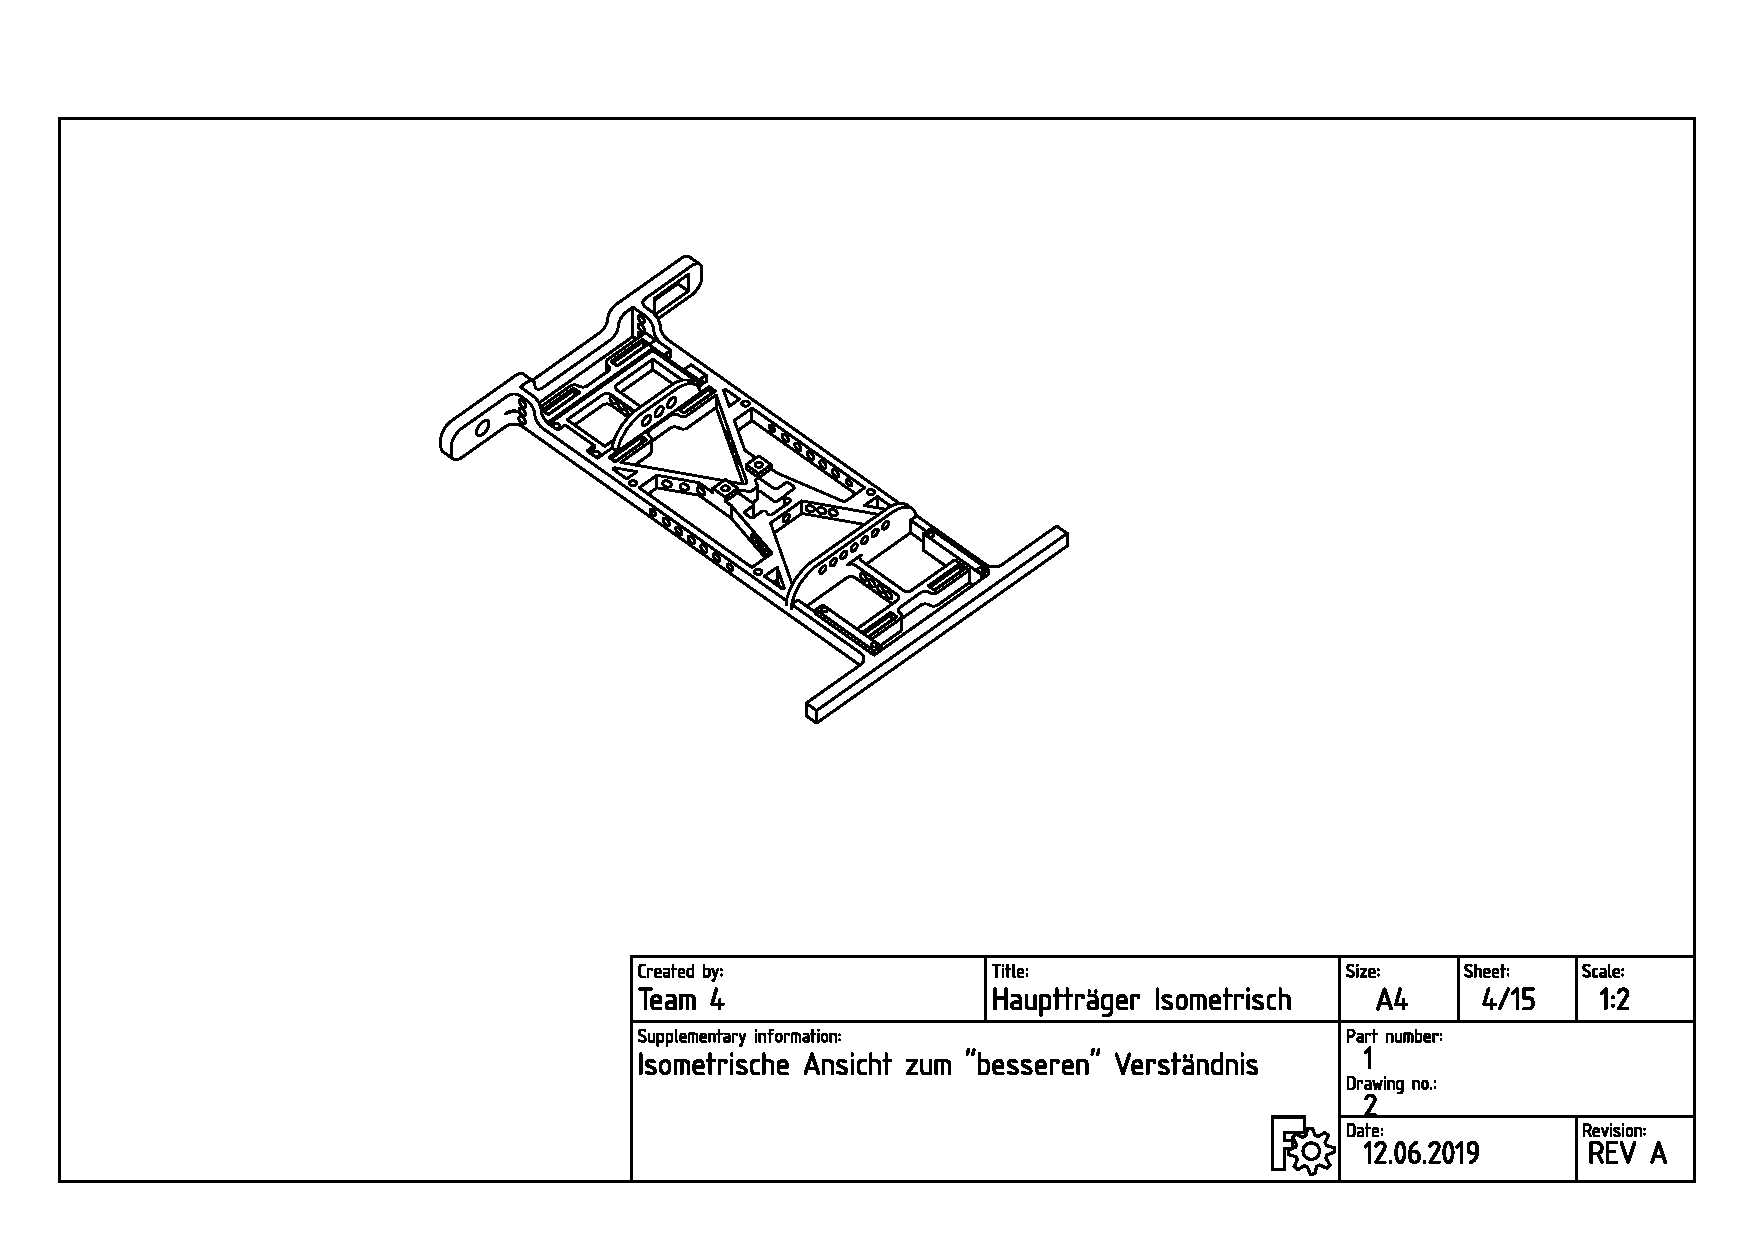
\includegraphics[width=\textwidth]{../techzeich/1iso.PDF} 	
	\caption{Haupttr�ger Isometrisch}
\end{figure}

\begin{figure}[ht!]
	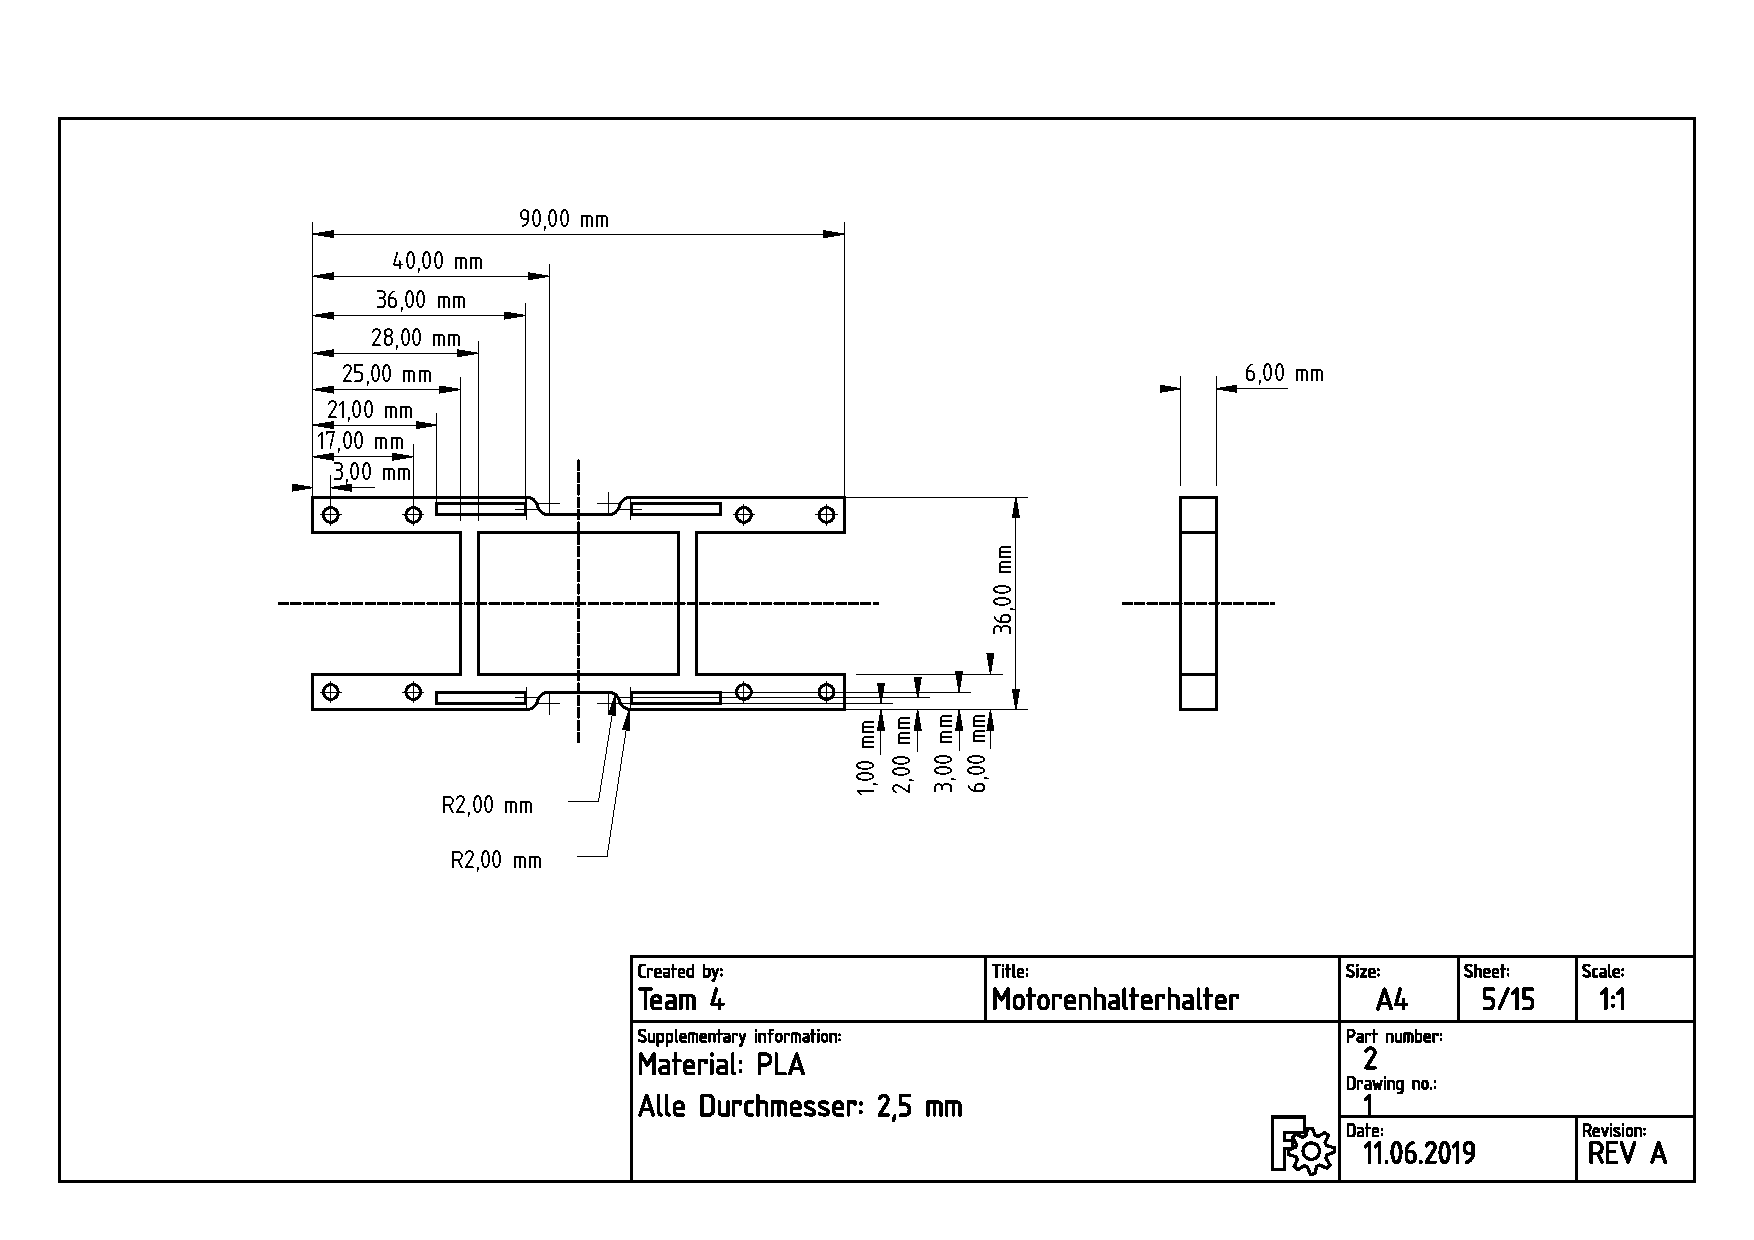
\includegraphics[width=\textwidth]{../techzeich/2.PDF} 	
	\caption{Motorenhalterhalter}
\end{figure}

\begin{figure}[ht!]
	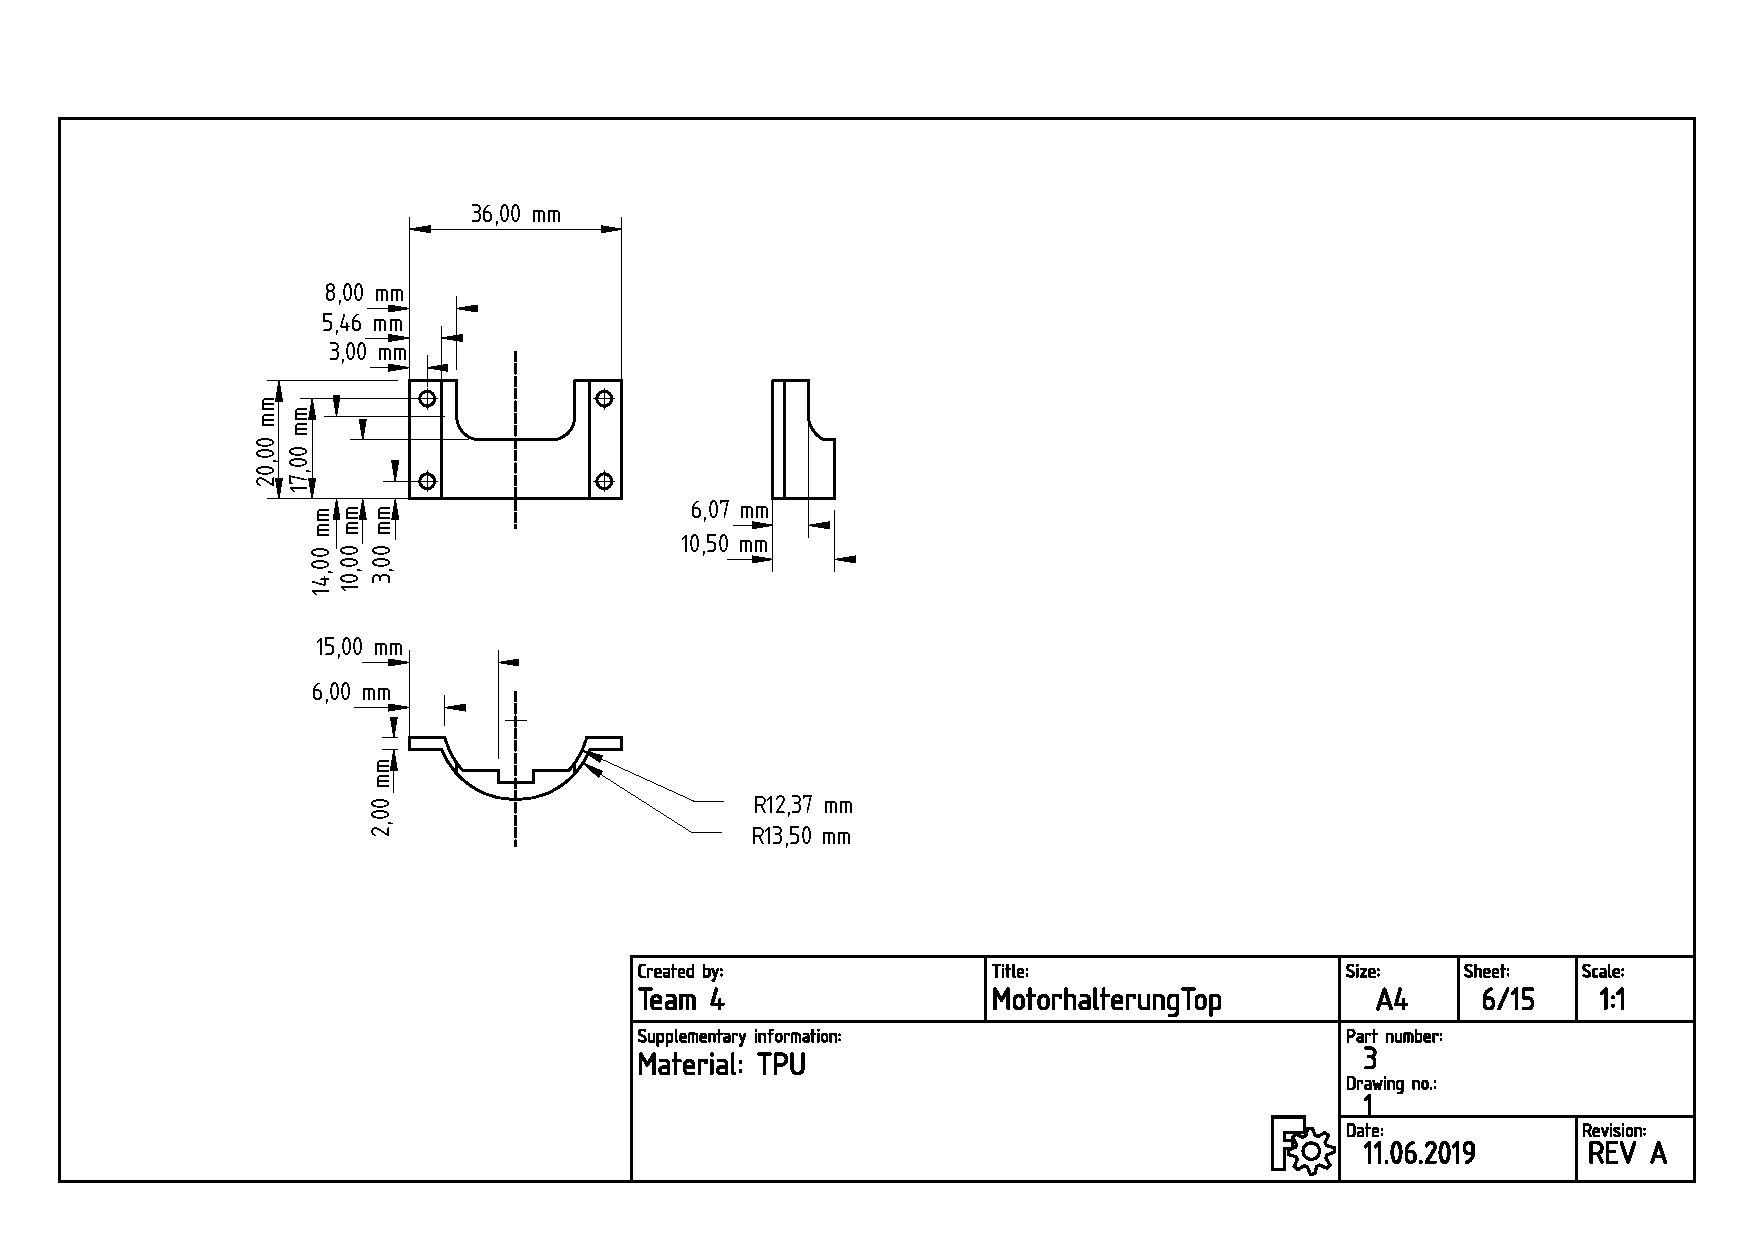
\includegraphics[width=\textwidth]{../techzeich/3.PDF} 	
	\caption{Motorenhalterung Oben}
\end{figure}
\begin{figure}[ht!]
	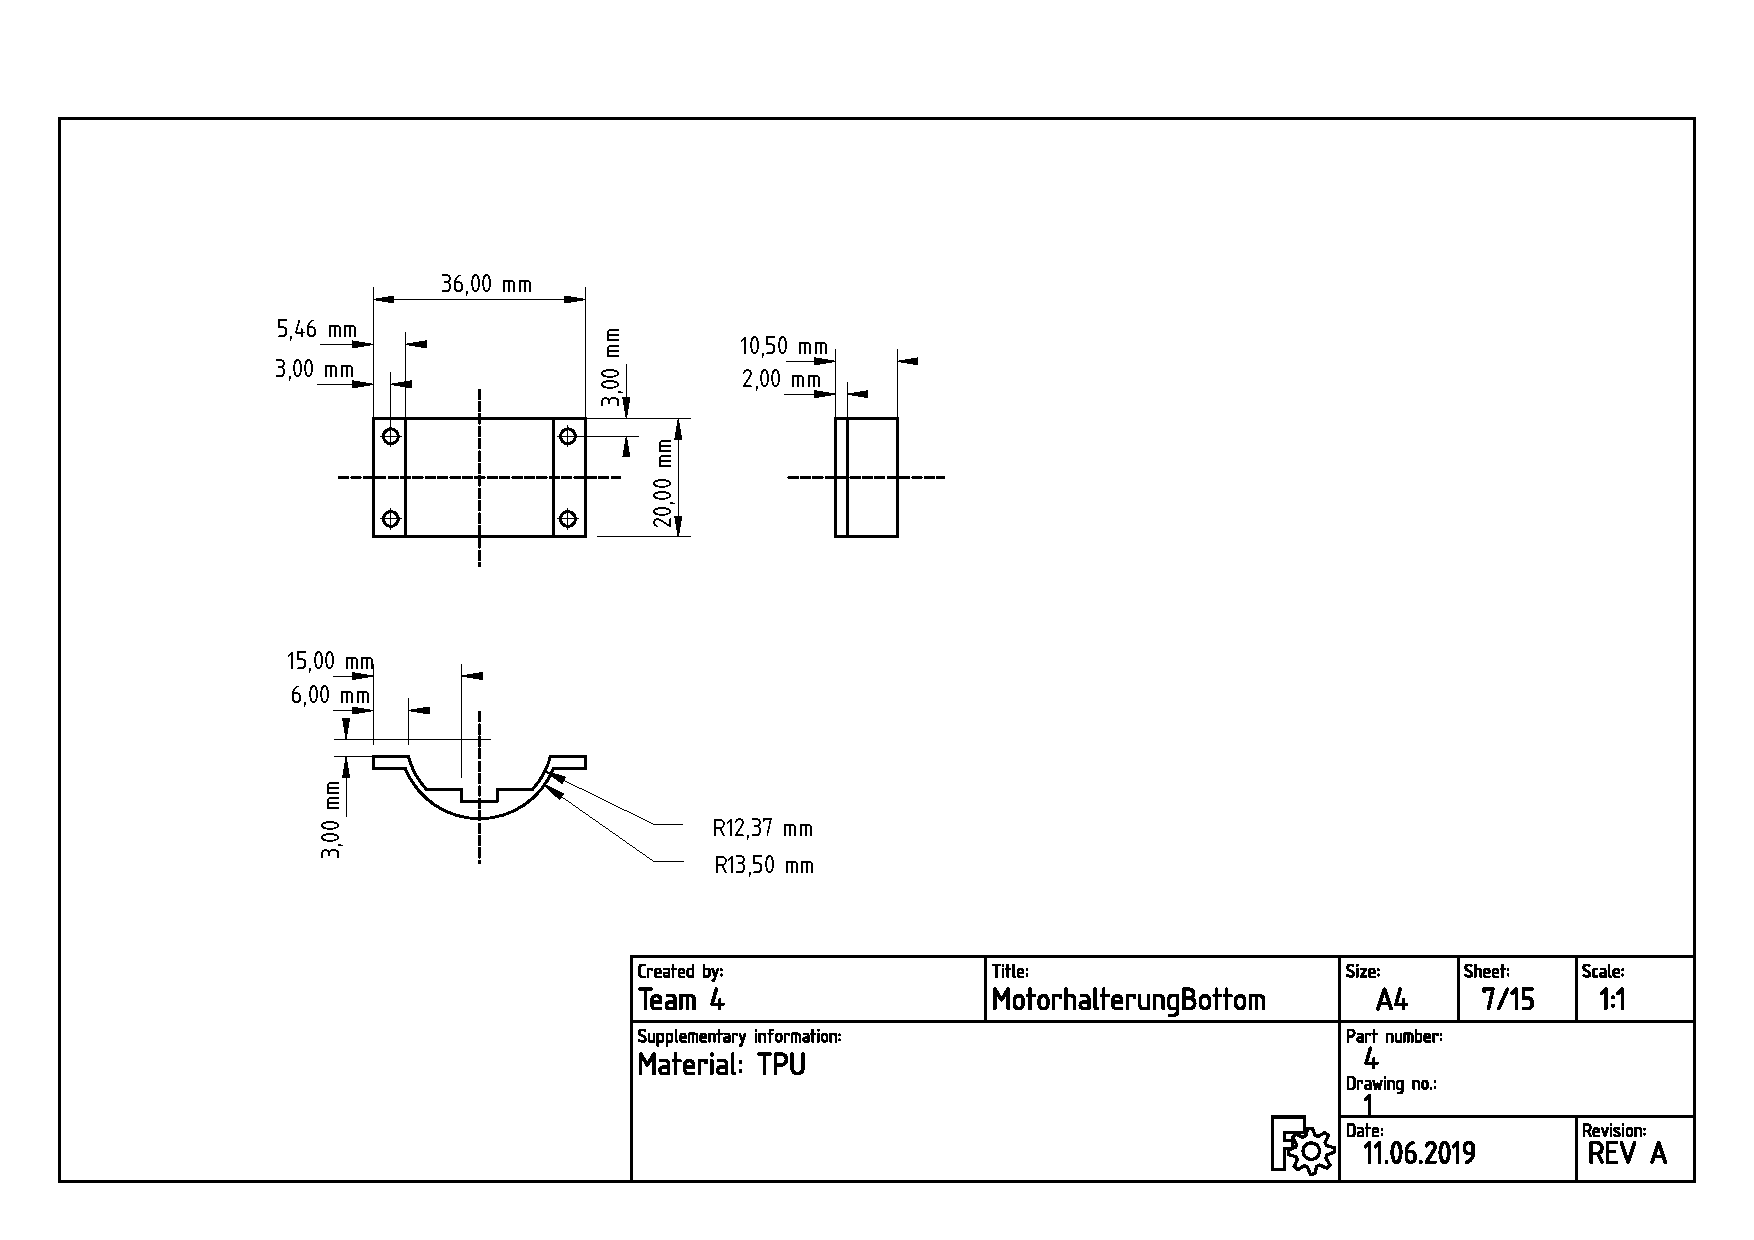
\includegraphics[width=\textwidth]{../techzeich/4.PDF} 	
	\caption{Motorenhalterung Unten}
\end{figure}
\begin{figure}[ht!]
	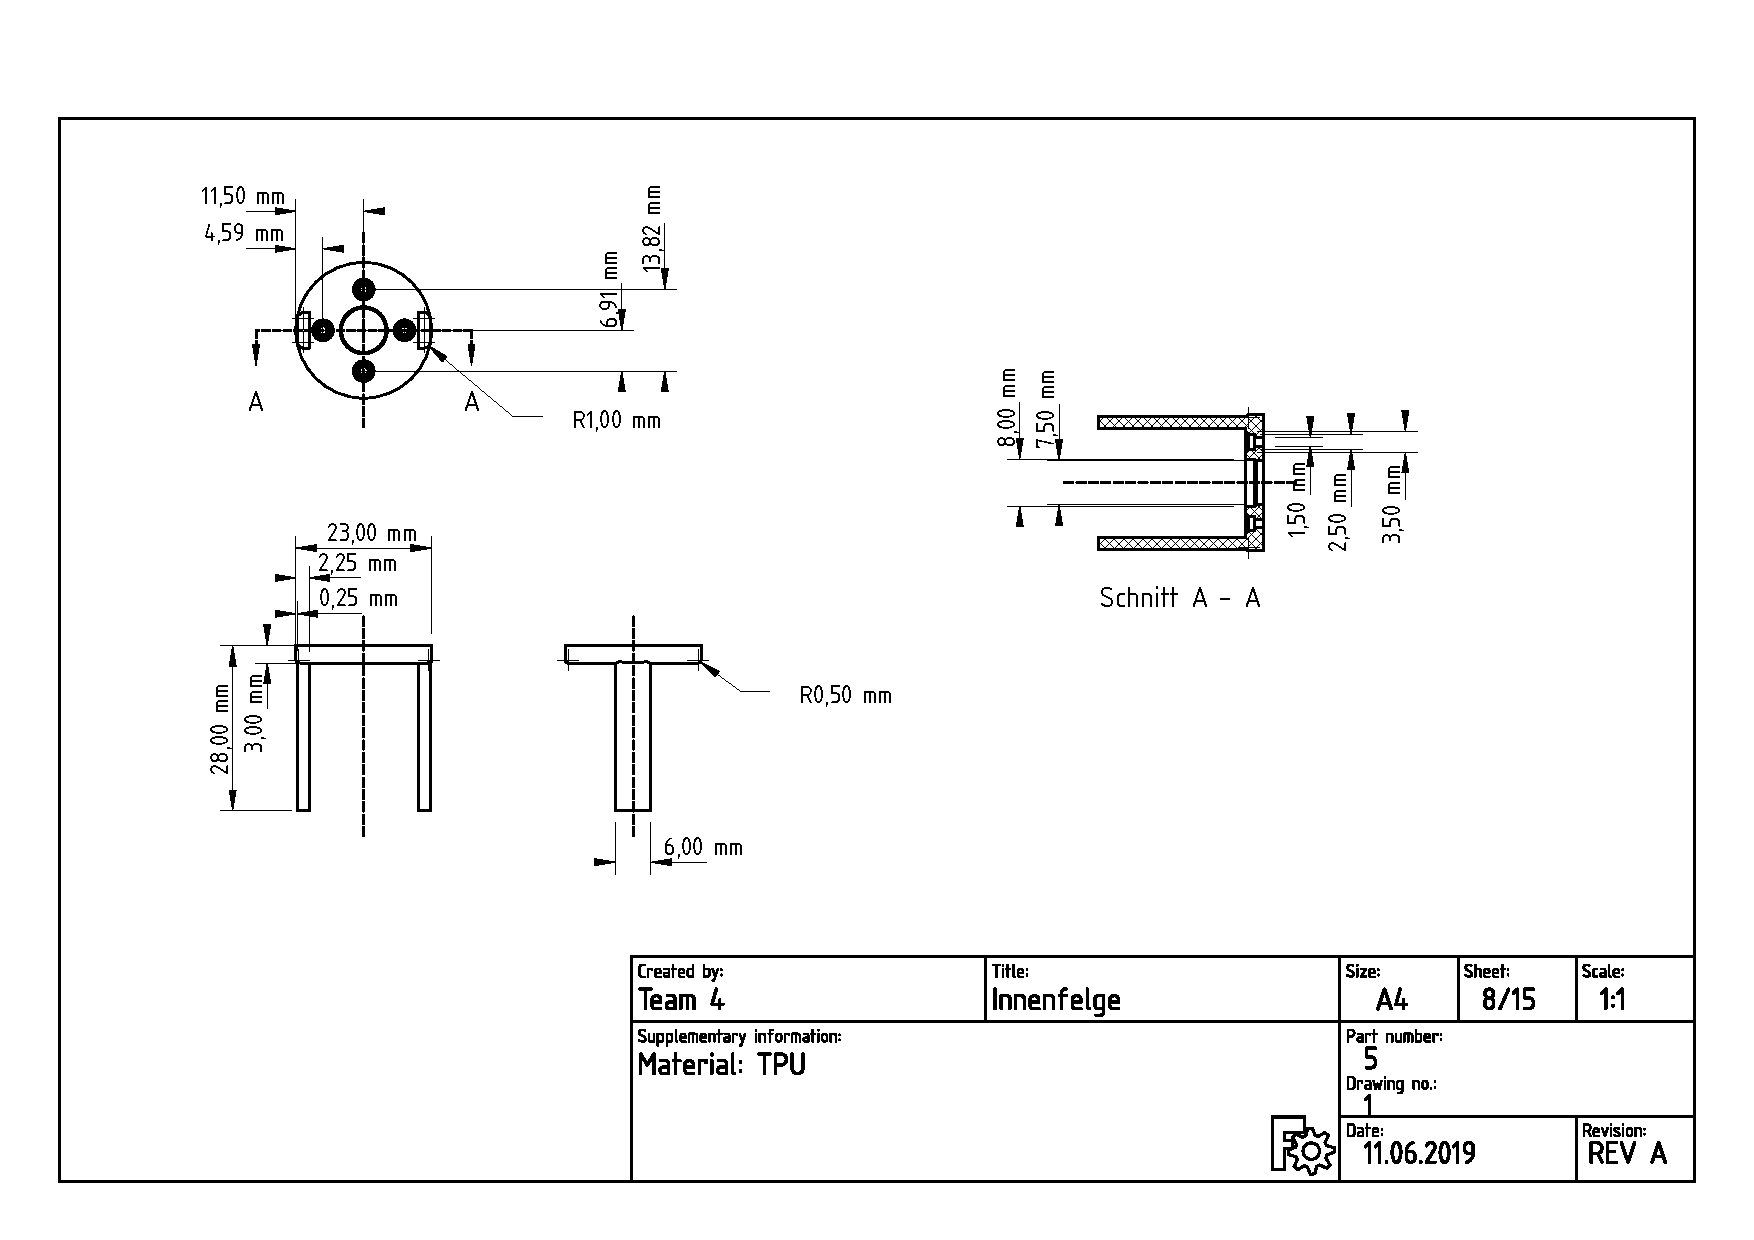
\includegraphics[width=\textwidth]{../techzeich/5.PDF} 	
	\caption{Innenfelge}
\end{figure}
\begin{figure}[ht!]
	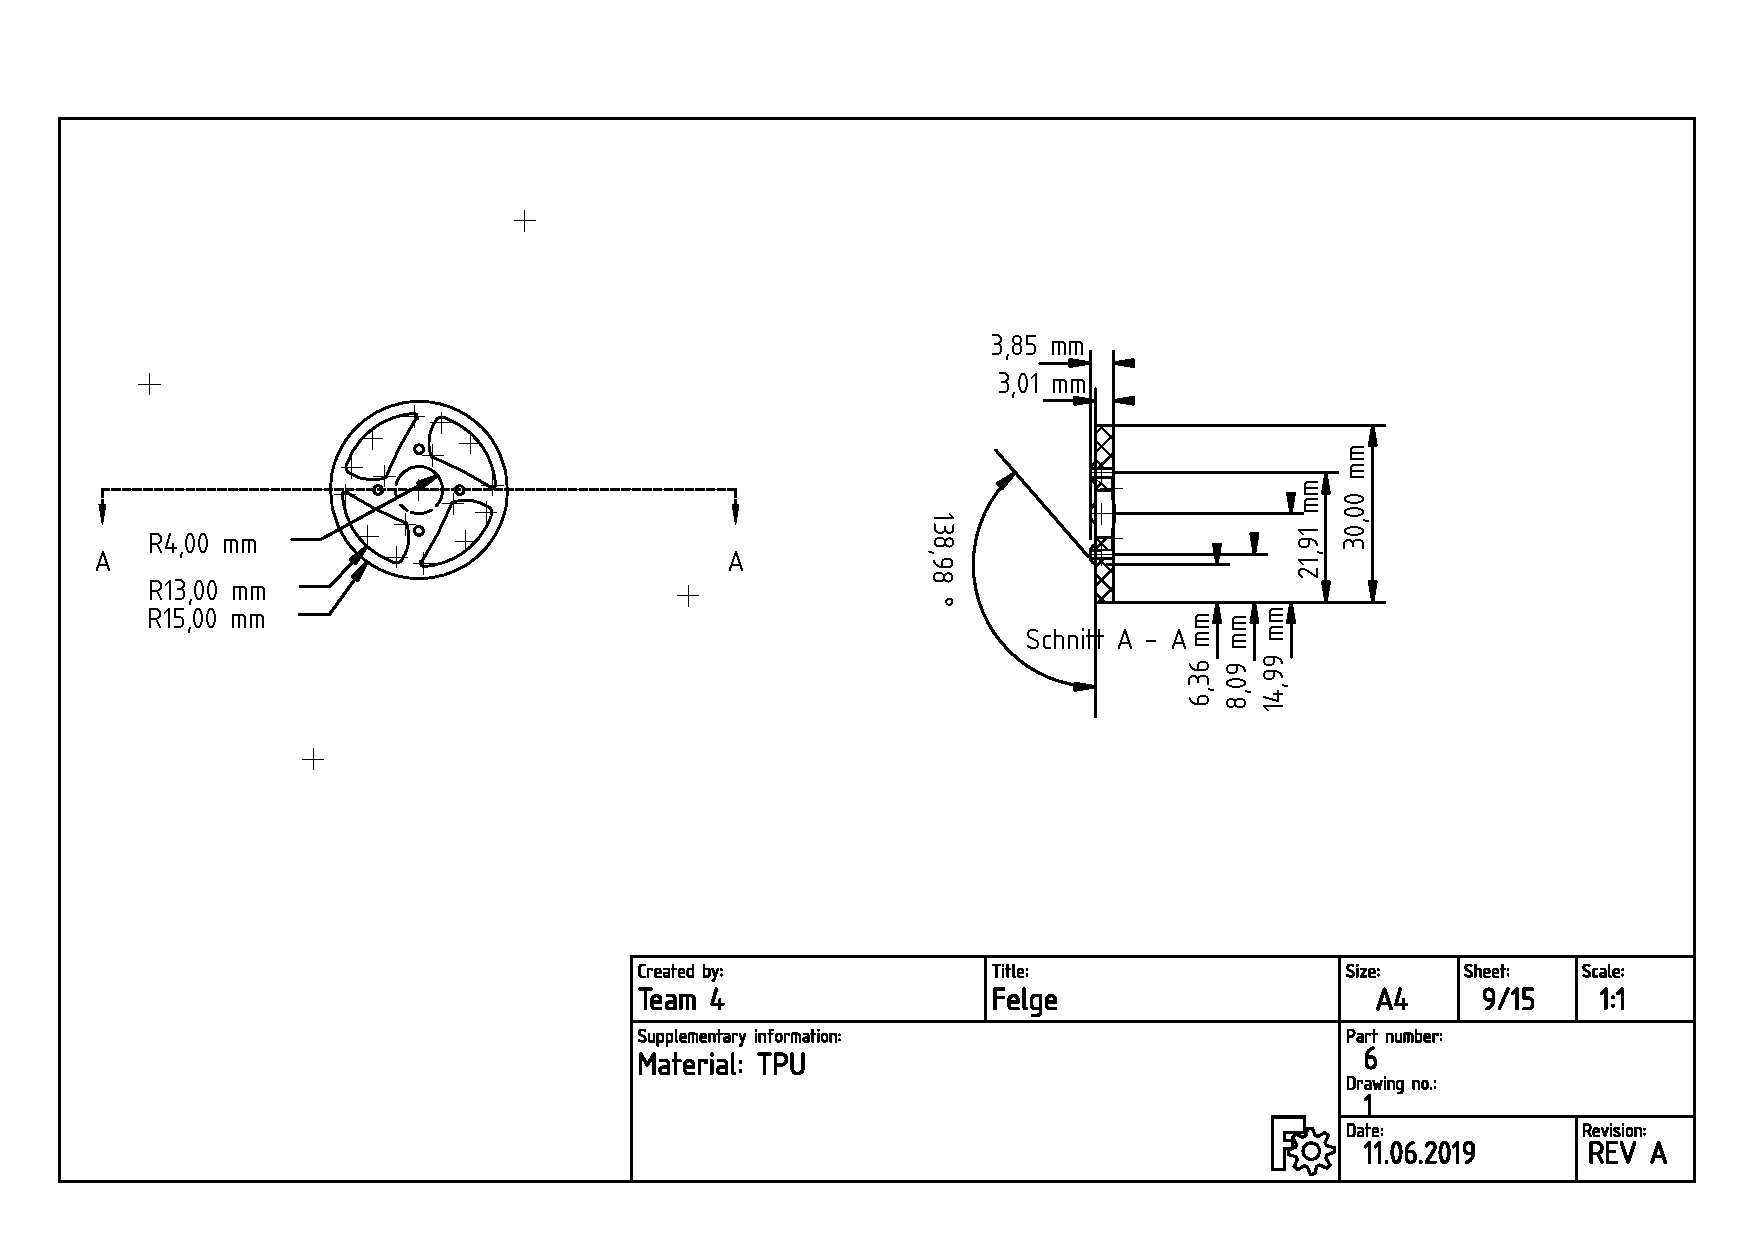
\includegraphics[width=\textwidth]{../techzeich/6.PDF} 	
	\caption{Felge}
\end{figure}
\begin{figure}[ht!]
	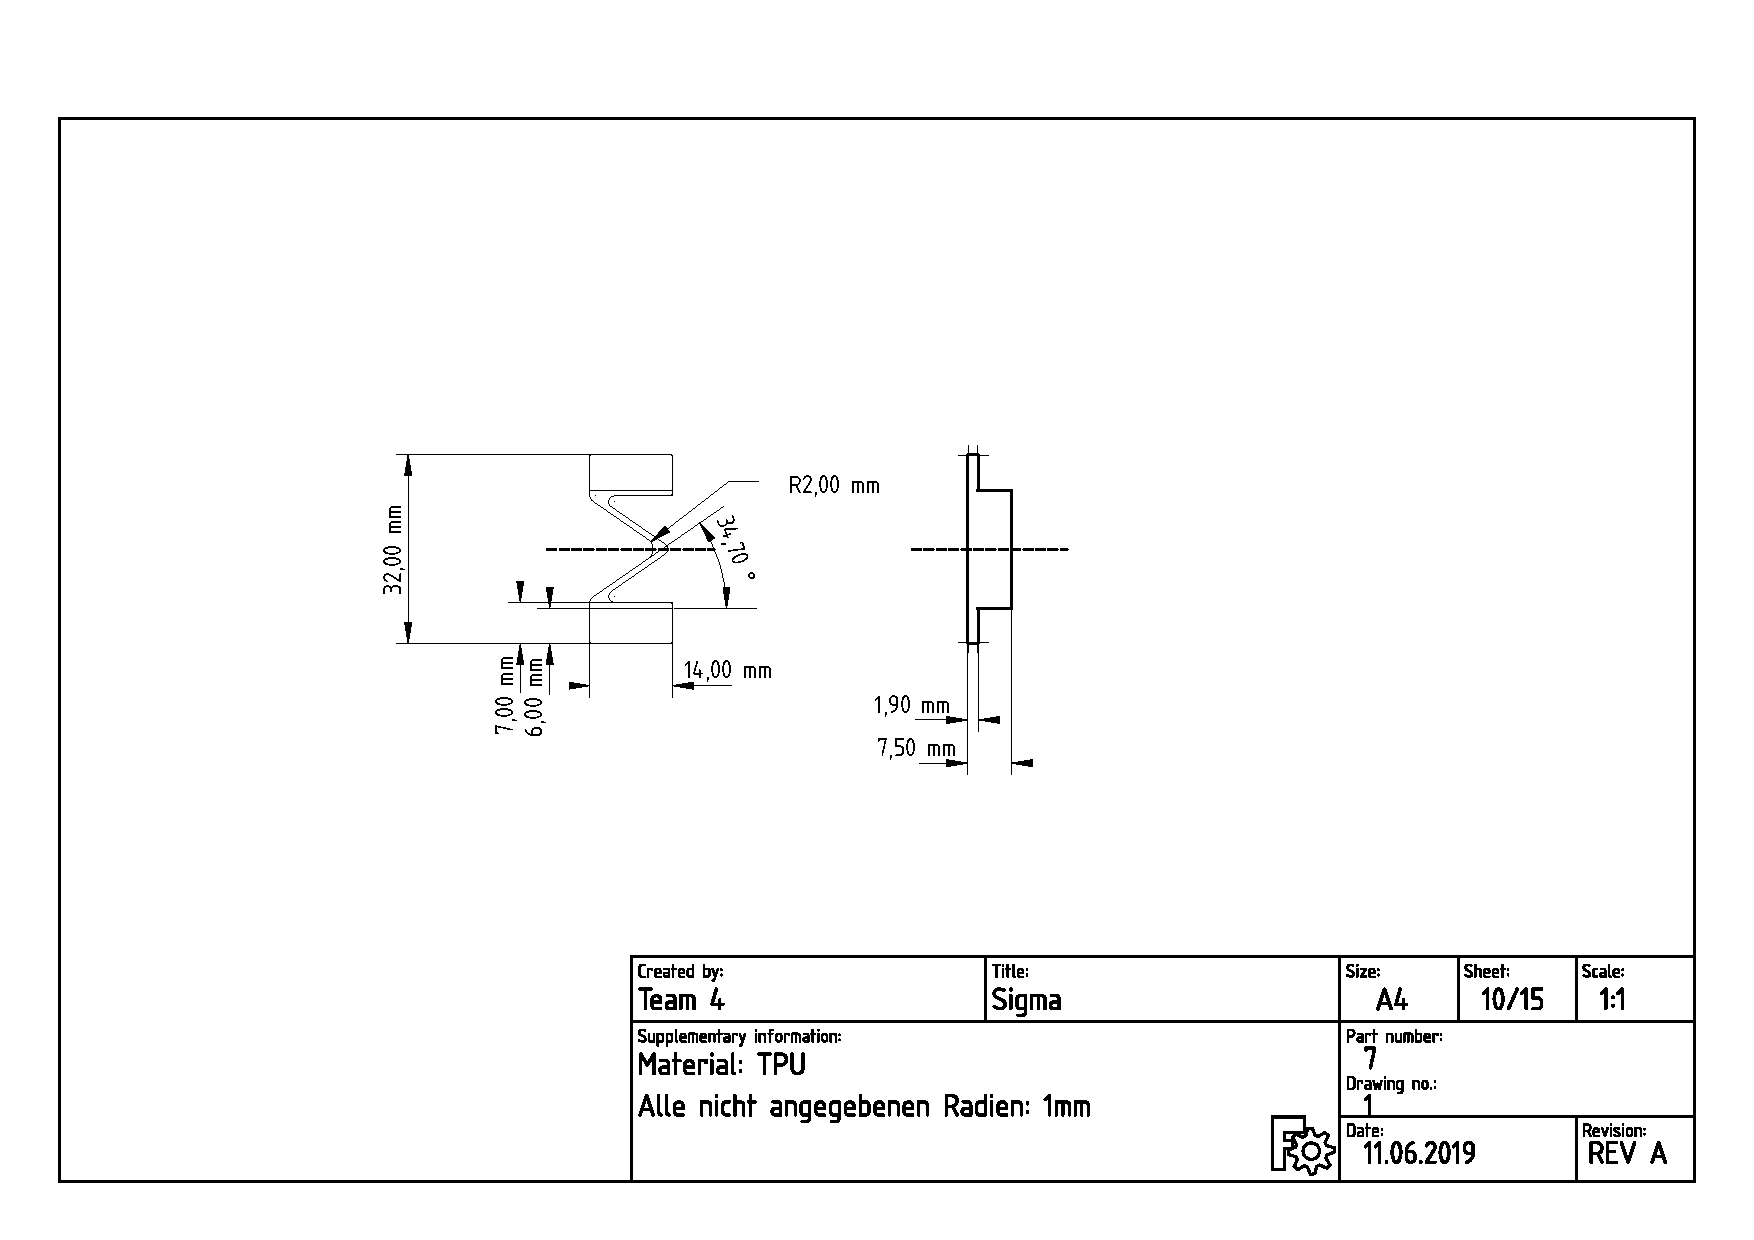
\includegraphics[width=\textwidth]{../techzeich/7.PDF} 	
	\caption{Sigma}
\end{figure}
\begin{figure}[ht!]
	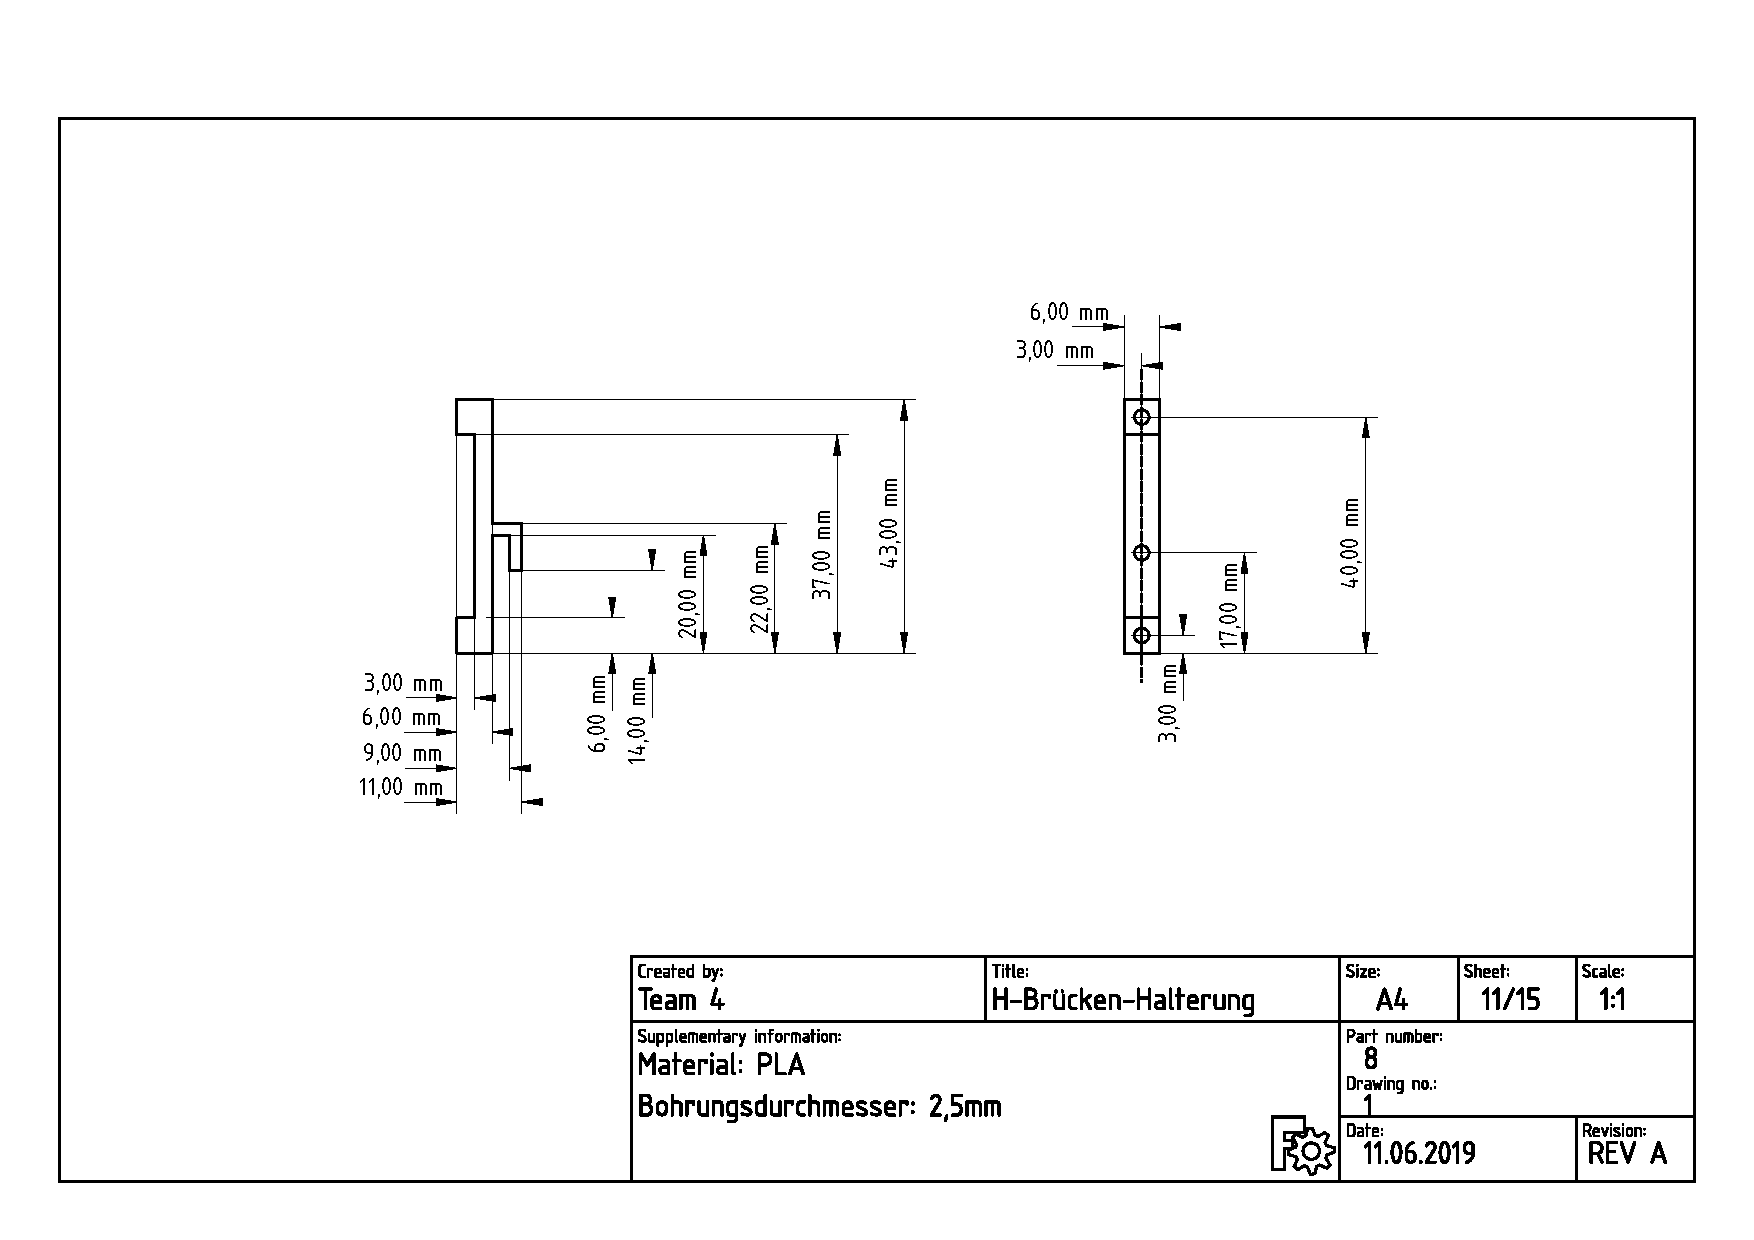
\includegraphics[width=\textwidth]{../techzeich/8.PDF} 	
	\caption{H-Br�cken-Halterung}
\end{figure}
\begin{figure}[ht!]
	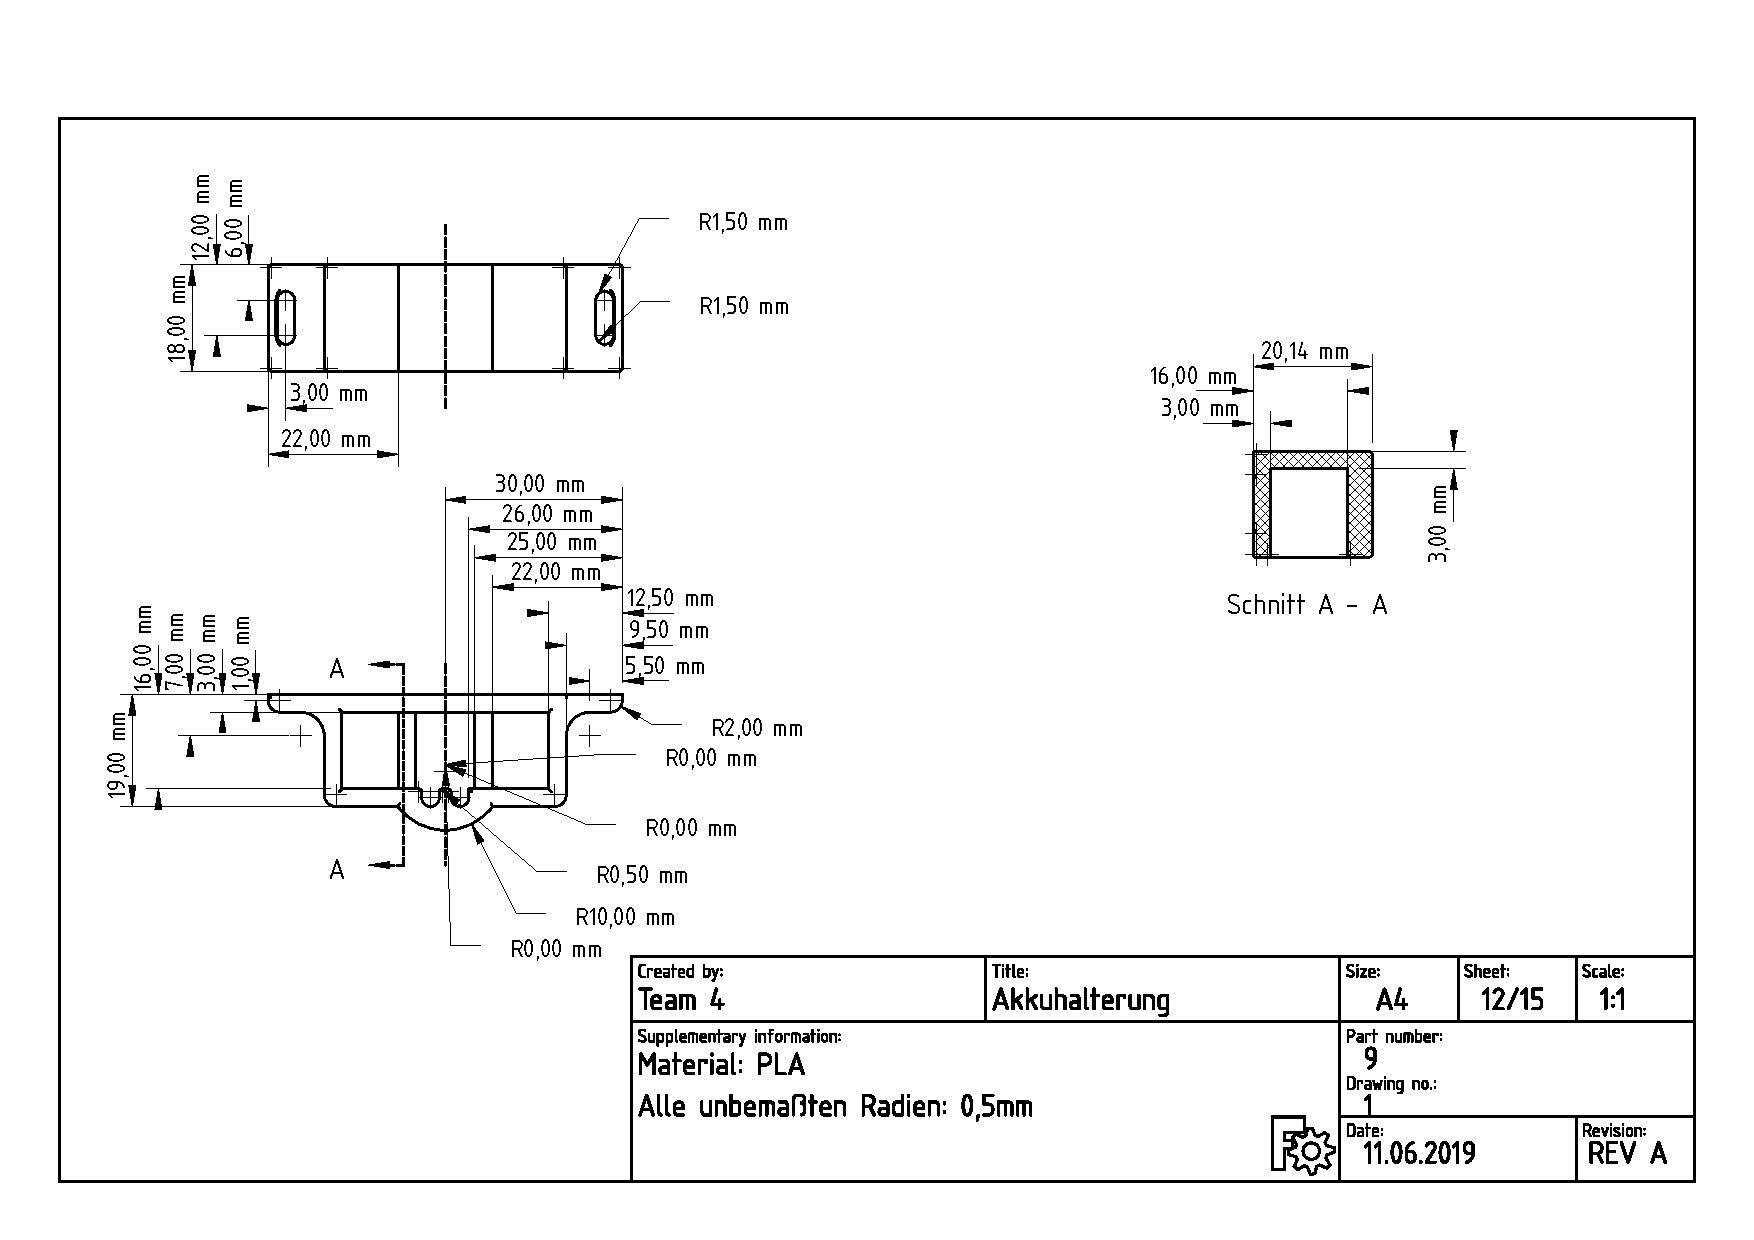
\includegraphics[width=\textwidth]{../techzeich/9.PDF} 	
	\caption{Akkuhalterung}
\end{figure}
\begin{figure}[ht!]
	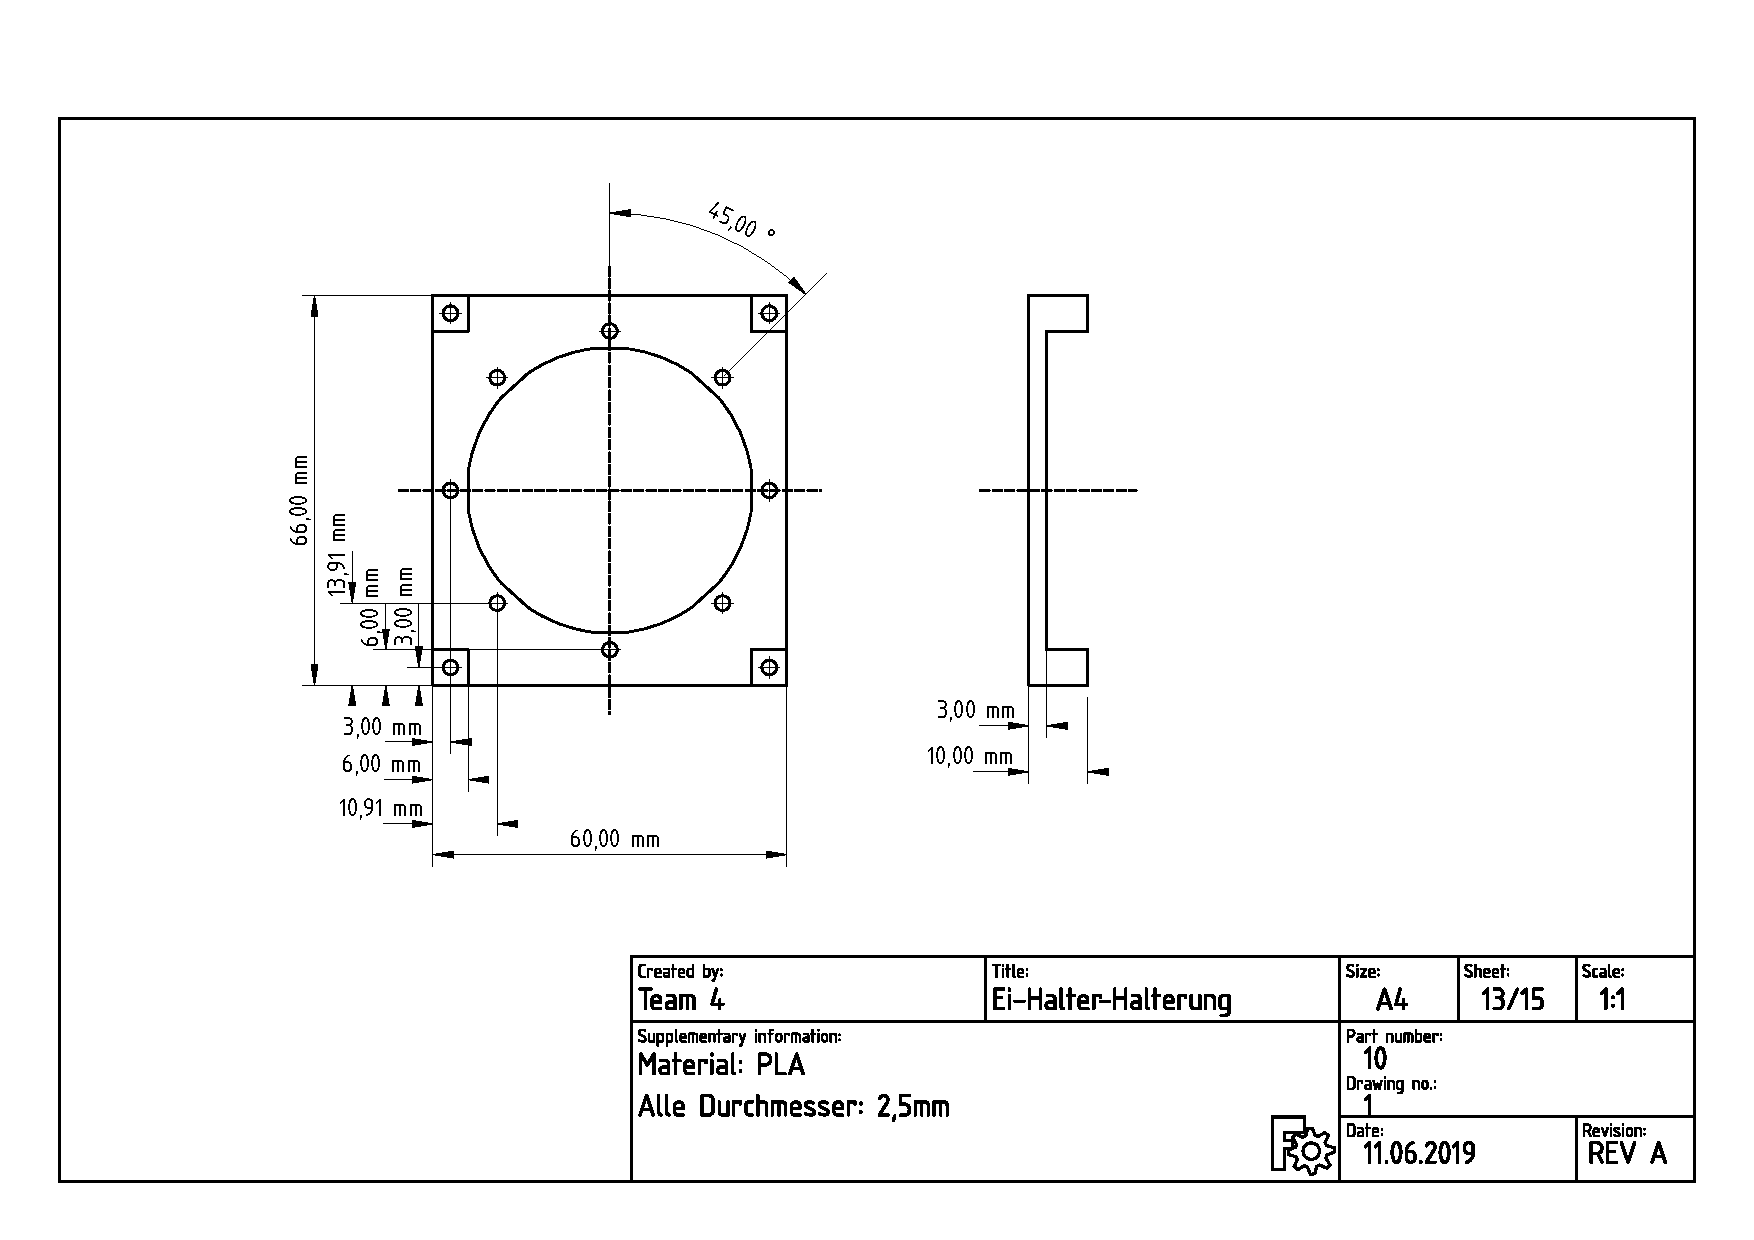
\includegraphics[width=\textwidth]{../techzeich/10.PDF} 	
	\caption{Ei-Halterung-Halterung}
\end{figure}
\begin{figure}[ht!]
	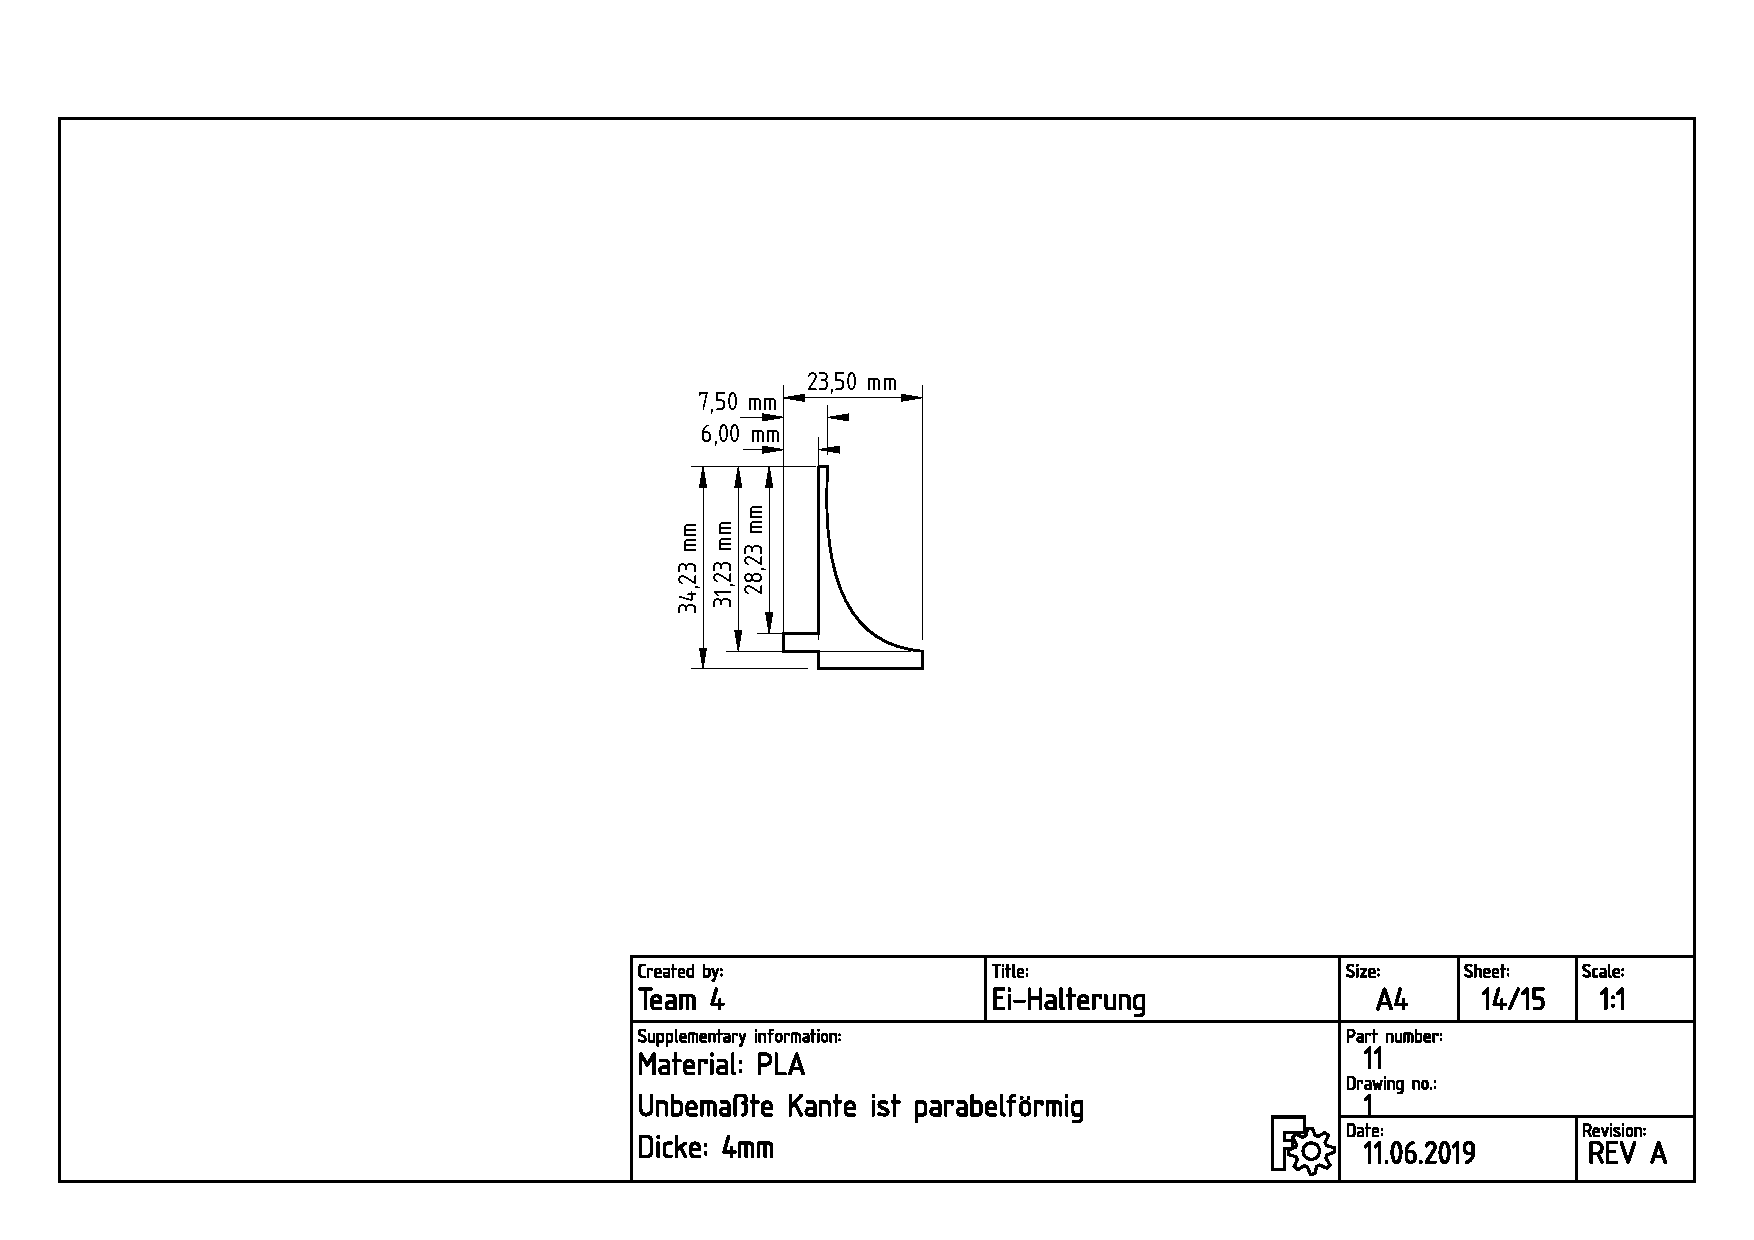
\includegraphics[width=\textwidth]{../techzeich/11.PDF} 	
	\caption{Ei-Halterung}
\end{figure}
\begin{figure}[ht!]
	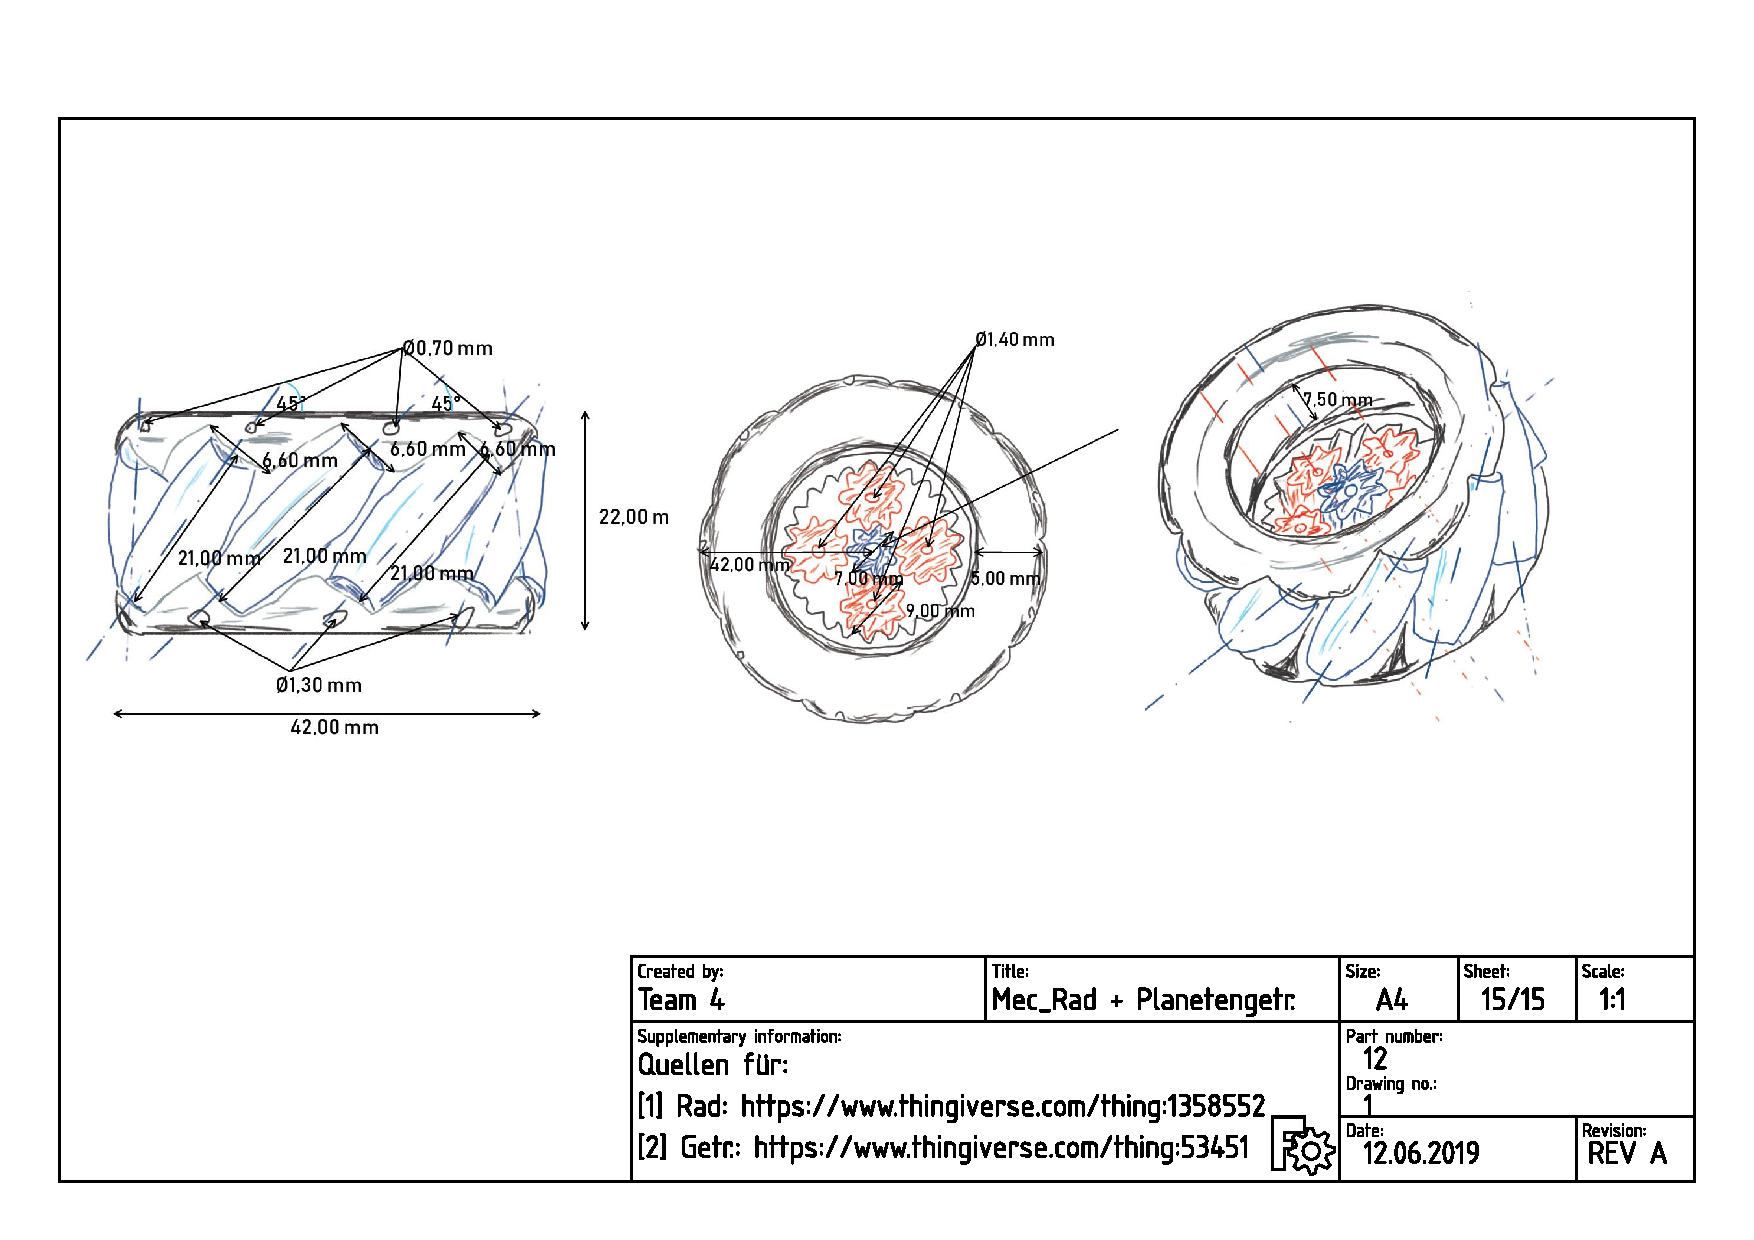
\includegraphics[width=\textwidth]{../techzeich/12.PDF} 	
	\caption{Reifen und Planetengetriebe}
\end{figure}

% Literaturverzeichnis einbinden
% %% ++++++++++++++++++++++++++++++++++++++++++++++++++++++++++++
%% Anhang: Literaturverzeichnis
%% ++++++++++++++++++++++++++++++++++++++++++++++++++++++++++++
%
%  Gerüst:
%  * Version 0.2
%  * Dipl.-Ing. Florian Evers, florian.evers@tu-ilmenau.de
%  * Fachgebiet Kommunikationsnetze, TU Ilmenau
%  * Dipl.-Ing. Christian Tolks, christian.tolks@informatik.uni-augsburg.de
%  * Lehrstuhl für Regelungstechnik, Universität Augsburg
%
%  Für Hauptseminare, Studienarbeiten, Diplomarbeiten
%
%  Autor           : Max Mustermann
%  Letzte Änderung : 31.12.2015
%

% Mit dem Befehl \nocite werden auch nicht im Text zitierte
% aus der Literaturdatenbank mit in das Literaturverzeichnis aufgenommen.
% Ein "\nocite{*}" übernimmt ungeprüft die komplette Datenbank.
%\nocite{*}

\cleardoublepage
\ihead[]{Literaturverzeichnis}
\bibliographystyle{plaindin} % oder {itmalpha}
\bibliography{literatur} % "literatur.bib" ist hier die einzige Literaturdatenbank.

% Alternativ: Mehrere Datenbanken verwenden, falls eine
% oder mehrere umfangreiche Sammlungen exisitieren:
%\bibliography{literatur_buecher,literatur_weblinks}



% Abbildungsverzeichnis einbinden
%% ++++++++++++++++++++++++++++++++++++++++++++++++++++++++++++
%% Anhang: Tabellenverzeichnis
%% ++++++++++++++++++++++++++++++++++++++++++++++++++++++++++++
%
%  Ger�st:
%  * Version 0.2
%  * Dipl.-Ing. Florian Evers, florian.evers@tu-ilmenau.de
%  * Fachgebiet Kommunikationsnetze, TU Ilmenau
%  * Dipl.-Ing. Christian Tolks, christian.tolks@informatik.uni-augsburg.de
%  * Lehrstuhl f�r Regelungstechnik, Universit�t Augsburg
%
%  F�r Hauptseminare, Studienarbeiten, Diplomarbeiten
%
%  Autor           : Max Mustermann
%  Letzte �nderung : 31.12.2015
%

% Hier keine weiteren �nderungen vornehmen
\cleardoublepage
\ihead[]{Aufz�hlungsverzeichnis}
\lstlistoflistings



% Abbildungsverzeichnis einbinden
%% ++++++++++++++++++++++++++++++++++++++++++++++++++++++++++++
%% Anhang: Abbildungsverzeichnis
%% ++++++++++++++++++++++++++++++++++++++++++++++++++++++++++++
%
%  Ger�st:
%  * Version 0.2
%  * Dipl.-Ing. Florian Evers, florian.evers@tu-ilmenau.de
%  * Fachgebiet Kommunikationsnetze, TU Ilmenau
%  * Dipl.-Ing. Christian Tolks, christian.tolks@informatik.uni-augsburg.de
%  * Lehrstuhl f�r Regelungstechnik, Universit�t Augsburg
%
%  F�r Hauptseminare, Studienarbeiten, Diplomarbeiten
%
%  Autor           : Max Mustermann
%  Letzte �nderung : 31.12.2015
%

% Keine �nderungen vornehmen!
\cleardoublepage
\ihead[]{Abbildungsverzeichnis}
\listoffigures


% Tabellenverzeichnis einbinden
%% ++++++++++++++++++++++++++++++++++++++++++++++++++++++++++++
%% Anhang: Tabellenverzeichnis
%% ++++++++++++++++++++++++++++++++++++++++++++++++++++++++++++
%
%  Gerüst:
%  * Version 0.2
%  * Dipl.-Ing. Florian Evers, florian.evers@tu-ilmenau.de
%  * Fachgebiet Kommunikationsnetze, TU Ilmenau
%  * Dipl.-Ing. Christian Tolks, christian.tolks@informatik.uni-augsburg.de
%  * Lehrstuhl für Regelungstechnik, Universität Augsburg
%
%  Für Hauptseminare, Studienarbeiten, Diplomarbeiten
%
%  Autor           : Max Mustermann
%  Letzte Änderung : 31.12.2015
%

% Hier keine weiteren Änderungen vornehmen
\cleardoublepage
\ihead[]{Tabellenverzeichnis}
\listoftables



% Abkürzungsverzeichnis einbinden
% %% ++++++++++++++++++++++++++++++++++++++++++++++++++++++++++++
%% Anhang: Abk�rzungsverzeichnis
%% ++++++++++++++++++++++++++++++++++++++++++++++++++++++++++++
%
%  Ger�st:
%  * Version 0.2
%  * Dipl.-Ing. Florian Evers, florian.evers@tu-ilmenau.de
%  * Fachgebiet Kommunikationsnetze, TU Ilmenau
%  * Dipl.-Ing. Christian Tolks, christian.tolks@informatik.uni-augsburg.de
%  * Lehrstuhl f�r Regelungstechnik, Universit�t Augsburg
%
%  F�r Hauptseminare, Studienarbeiten, Diplomarbeiten
%
%  Autor           : Max Mustermann
%  Letzte �nderung : 31.12.2015
%

% Hier keine weiteren �nderungen vornehmen
\cleardoublepage
\ihead[]{Abk�rzungsverzeichnis und Formelzeichen}
\printnomenclature



% Thesen
% %% ++++++++++++++++++++++++++++++++++++++++++++++++++++++++++++
%% Thesen zur Ausarbeitung. F�r Diplomarbeiten
%% ++++++++++++++++++++++++++++++++++++++++++++++++++++++++++++
%
%  Ger�st:
%  * Version 0.10
%  * Dipl.-Ing. Florian Evers, florian.evers@tu-ilmenau.de
%  * Fachgebiet Kommunikationsnetze, TU Ilmenau
%
%  F�r Hauptseminare, Studienarbeiten, Diplomarbeiten
%
%  Autor           : Max Mustermann
%  Letzte �nderung : 31.12.2015
%

\chapter*{Thesen zur \artderausarbeitung}
\addcontentsline{toc}{chapter}{Thesen zur \artderausarbeitung}
\ihead[]{Thesen zur \artderausarbeitung}

\begin{enumerate}
\item Mit \LaTeX\ gesetzte Dokumente sehen �berall
      gleich aus. Sie werden �hnlich wie HTML in Klartext
      geschrieben und anschlie�end mit Hilfe eines Konverters in
      Postscript- oder PDF"=Dateien gewandelt.
\item \LaTeX\ gibt es f�r alle wichtigen Betriebssysteme.
\item Die Benutzung einer integrierten Entwicklungsumgebung,
      beispielsweise {\ttfamily Kile} oder {\ttfamily TeXnicCenter},
      wird empfohlen.
\item Dieses Dokument ist Formatvorlage und Einstiegshilfe
      zugleich. Einfach den Text durch die eigene Ausarbeitung
      ersetzen.
\end{enumerate}

% Etwas Platz schaffen:
\section*{}

Ilmenau, den 31.\,12.\,2015\hfill \namedesautors


% Abschlusserklärung
% %% ++++++++++++++++++++++++++++++++++++++++++++++++++++++++++++
%% Vorwort: Abschlusserkl�rung
%% ++++++++++++++++++++++++++++++++++++++++++++++++++++++++++++
%
%  Ger�st:
%  * Version 0.2
%  * Dipl.-Ing. Florian Evers, florian.evers@tu-ilmenau.de
%  * Fachgebiet Kommunikationsnetze, TU Ilmenau
%  * Dipl.-Ing. Christian Tolks, christian.tolks@informatik.uni-augsburg.de
%  * Lehrstuhl f�r Regelungstechnik, Universit�t Augsburg
%
%  F�r Hauptseminare, Studienarbeiten, Diplomarbeiten
%
%  Autor           : Max Mustermann
%  Letzte �nderung : 31.12.2015
%

\chapter*{Erkl�rung}
\addcontentsline{toc}{chapter}{Erkl�rung}
\ihead[]{Erkl�rung}

Die vorliegende Arbeit habe ich selbstst�ndig ohne Benutzung anderer als der
angegebenen Quellen angefertigt. Alle Stellen, die w�rtlich oder sinngem��
aus ver�ffentlichten Quellen entnommen wurden, sind als solche
kenntlich gemacht. Die Arbeit ist in gleicher oder �hnlicher Form oder
auszugsweise im Rahmen einer oder anderer Pr�fungen noch nicht vorgelegt
worden.
\\[2cm]
Ilmenau, den 31.\,12.\,2016\hfill \namedesautors


\end{document}

